\chapter{Design and Implementation} \label{chapter:design-and-implementation}

The design and implementation chapter documents the practical part of the thesis.
It is comprised of two sections, namely the extension of the original standalone neural
    ranking model to be usable with the MSMARCO passage ranking dataset,
    as well as the migration of the SNRM's source code from the Python library TensorFlow 
    to PyTorch.
The reproduction of the original work from 
    Zamani et al. \cite{zamani:2018:from-neural-reranking-to-neural-ranking}
    using the MSMARCO dataset represents also a primary objective.
Each of these sections describes in chronological order the realized
    design and implementation tasks, encountered challenges, 
    carried out experiments and also their results.\\
Zamani et al. provide the source code of their standalone neural ranking model as a
    repository on GitHub
    \footnote{Hamed Zamani's SNRM GitHub repository \url{https://github.com/hamed-zamani/snrm}}
    under the BSD-3-Clause license.
A fork of the original SNRM GitHub repository was created
    \footnote{Bernhard Steindl's fork \texttt{"snrm-extension"} of the original SNRM GitHub repository \url{https://github.com/Bernhard-Steindl/snrm-extension}}
    and used as the code basis.
Under the forked repository \texttt{"snrm-extension"}, two git branches were created.
The first branch \texttt{"extension"} contains the source code changes concerning the first
    section of the SNRM reproducibility and extension.
Secondly, the branch \texttt{"extension-pytorch"} comprises the realization of the migration
    from TensorFlow to PyTorch, according to the second section of this chapter.

% TODO make forked GitHub repo code public!

\section{SNRM reproducibility and extension}
This section describes the taken steps to set-up the original standalone neural ranking model of Zamani et al.
    and to extend and modify the project to be able to use the MSMARCO passage ranking dataset.
According to the SNRM paper of Zamani et al. \cite{zamani:2018:from-neural-reranking-to-neural-ranking} 
    datasets of Robust (TREC), ClueWeb, and AOL query logs, as well as a Wikipedia dump was used
    in their work.
However, the lack of these datasets led to the use of the MSMARCO datasets, 
    and due to its free availability for non-commercial research purposes.

\subsection{Setup original SNRM implementation}
At the beginning, the original TensorFlow implementation of SNRM was examined and studied,
    before setting the project up on an Apple MacBook Pro (Retina, 15-inch, Mid 2015).
The first objective was to make the original SNRM application runnable on this local system.
Unfortunately, the authors neither stated the versions of Python, TensorFlow and NumPy on their paper nor 
    in the SNRM GitHub repository.
Hence, the first effort was put in trying different versions and resolve version conflicts between dependencies.
By trial-and-error executing SNRM TensorFlow with various versions, the following versions seemed to make the   
    application run.
Probable, these versions were used by the authors of he SNRM with TensorFlow:
\begin{itemize}
    \item python 3.6.9
    \item tensorflow 1.4.0
    \item numpy 1.16.4
\end{itemize}
It is even probable that a Python version below 3 was used, due the author's usage of the Python 
    function \texttt{xrange} in the source code, which did exist in Python 2, but was removed in Python version 3.
After finding potential suitable Python, TensorFlow and NumPy versions, runtime errors occured, likely due to 
    invokations of incompatible resp. obsolete api methods and attributes by the SNRM code.

\subsection{Modification of dictionary for tokenization, stopword filter}
SNRM's \texttt{code/dictionary.py} opens a file comprising tokens and generates two datastructures, one for mapping 
    from an id to a token, and vice versa.
According to the original SNRM source code, the authors loaded vocabulary terms from the output of 
    Galago's \verb|dump_term_stats| function.
There was no reference supplied where to download their vocabulary terms.
Hence, the file \verb|allen_vocab_lower_10/tokens.txt| from the Advanced Information Retrieval course's exercise files 
    \footnote{Advanced IR course's excercise files \url{https://owncloud.tuwien.ac.at/index.php/s/QA4LEtxdBokqdNx}}
    was chosen and used as a token file and in this way the known vocabulary.
The original implementation for loading the vocabulary tokens had to be adjusted due to a different format of the token file.
It is worth to note, that the original SNRM implementation only used simple whitespace (\verb|" "|) tokenization.
Instead of retaining the simple whitespace tokenization, NLTK word tokenization was employed.
NLTK in version 3.4.5, a Python dependency, was added for using the NLTK corpus' english stopwords and word tokenization.
The file \texttt{code/dictionary.py} was edited and the function \verb|get_term_id_list| was added as a 
    replacement of the previous tokenization technique, for the means to generate a list of term-ids from 
    query and document text via word tokenization with regards to remove stop words, too.

\subsection{Implementation of batch data provisioning}
The paper's authors did not provide the function \verb|generate_batch| within the python file \verb|code/train.py|, 
    which is supposed to be used for generating a new batch of training data (resp. validating data), while 
    also remembering which data was already generated.
One raw batch is a matrix comprising various query texts, two document texts (passages), and a label indicating which document 
    is more relevant to the corresponding query text.
The batch data's query and document text have to be represented as term ids. 
As a consequence, the positve and negative document as well as the query texts had to be tokenized, stopwords had be removed,
    and the representations had to be trimmed or padded to have a common length.

\todo{@Sebastian: Wie wurde das AIR triples.train.tsv file generiert? Sollen wir das erwähnen?}
Concerning training and validation data, at first a processed subset of the MS MARCO dataset was used, 
    \verb|triples.train.tsv| (ca. 1.7 GB), which was downloaded from the Advanced IR course's exercise files.
The triples file was split in two distinct files, namely one for training and the other for validation data.
The format of the dataset is \verb|"query \t relevant-doc \t non-relevant-doc"|.

The SNRM model was operated with pre-trained GloVe word vectors
    \footnote{GloVe pre-trained word vectors GitHub repository \url{https://github.com/stanfordnlp/GloVe\#download-pre-trained-word-vectors}},
    which were downloaded from their GitHub repository.
Different GloVe embeddings were used for experimenation, namely \verb|glove.42B.300d.txt|, 
    of corpora Common Crawl (42B tokens, 1.9M vocab, uncased, 300d vectors, 1.75 GB download), 
    and \verb|glove.6B.100d.txt|, of corpora Wikipedia 2014 + Gigaword 5 (6B tokens, 400K vocab, uncased, 100d vectors, 822 MB download).

Similarly, the authors of the SNRM paper did not implement the \verb|generate_batch| function for the phase of index construction in 
    the file \verb|code/index_construction.py|. As a result, the function had to be implemented in such a way, that it returns a
    batch resp. matrix comprising of multiple document-id entries and assigning every document-id a list of the document token ids.
    The document token ids were obtained the same way as in the training phase's batch generation 
    (tokenization, stopword removal, padding/trimming).
As the data source for generating passage text batches, the document collection \verb|collection.tsv| (ca. 2.9 GB)
    \footnote{MS MARCO passage ranking document collection dataset download link 
    \url{https://msmarco.blob.core.windows.net/msmarcoranking/collection.tar.gz}}, 
    from the MS MARCO passage ranking GitHub repository was used, which has the format \verb|"passage-id \t passage-text"|.

For the reader it remains unclear, why the source code for batch generation has been deleted and replaced with an exception 
    pointing out the missing implementation. 
Probably, the code was too domain-specific or too closely tied to the chosen training data and document collection,
    so it was not worth making it publicly available on GitHub.
Nevertheless, for the reproduction of the SNRM's results it is necessary to add the lacking implementation details.

\subsection{Customization of the retrieval and evaluation script}
The authors' script for the retrieval phase (\texttt{code/retrieval.py}) had only hard-coded two example queries,
    and demonstrated the steps resp. the concept for obtaining the retrieval scores for documents, for a given query.
After mapping the query text to a list of token ids, generation of a latent query representation vector through model inference, 
    inverted index lookup for relevant documents with the latent representation's dimension, a document's retrieval score was
    calculated by summation over a document's latent term weigh and the coefficient of the corresponding latent query term dimension.
Afterwards, the original SNRM code just writes the document retrieval scores to a binary file by Pyhon object 
    serialization (\texttt{pickle}).
One of the goals in reproducing the paper and the source code, was to evaluate the retrieval model with recent evaluation tools like 
    \verb|trec_eval| \footnote{Evaluation software \texttt{trec\_eval} GitHub repository \url{https://github.com/usnistgov/trec_eval}},
    and \verb|msmarco_eval.py| 
    \footnote{Evaluation software \texttt{msmarco\_eval.py} GitHub repository \url{https://github.com/spacemanidol/MSMARCO/blob/master/Ranking/Baselines/msmarco_eval.py}}.
Associated with this, the retrieval Python script was modified, to process as input a query file, to write the retrieval result as an 
    evaluation file comprising the retrieved and relevant document candidates in TREC format, 
    and to allow to stop retrieval after a configurable number of input queries have been processed. 

The MS MARCO passage ranking GitHub repository also provides queries and TREC qrel files for model evaluation.
As a starting point, the query file \texttt{queries.dev.small.tsv} and the qrel file \texttt{qrels.dev.small.tsv} were downloaded
    \footnote{MS MARCO passage ranking queries, and qrel files download link \url{https://msmarco.blob.core.windows.net/msmarcoranking/collectionandqueries.tar.gz} }.
    and used.

By writing and utilizing a Python script for analysing the qrel file's content, the following statistics have been observed.
The qrel file \texttt{qrels.dev.small.tsv} comprises of 6,980 queries in total.
When grouping all queries by how much relevant documents a certain query has, as a result is obtained, that 
    out of all queries, 6,590 queries have only one relevant document, resp. 331 queries have two, 
    51 queries have three and 8 queries have four relevant documents, accoding to the relevance judgements file.

\subsection{Creation of a Google Colab notebook}
Unfortunately, the own available personal computers lack the accessibility to a NVIDIA GPU.
NVIDIA GPUs proved to be well equipped for improving model training performance and speed, compared to a CPU.
Hence, after making the original SNRM code with stated modifications executable, a Google Colab notebook was created
    with Google Colaboratory (Colab) 
    \footnote{Google Colaboratory (Colab) website \url{https://colab.research.google.com}},
    for executing the SNRM application phases in a Jupyter Notebook like environment, 
    but also utilizing a free NVIDIA GPU.
In the Google Colab Notebook, commands were used to setup the platform (NVIDIA CUDA, NVIDIA cuDNN, Miniconda, pip, Python, etc.),
    checkout the GitHub source code,
    install the required project dependencies, downloading and extracting datasets,
    before invoking the Python scripts, according to the model's information retrieval phases
    model training, inverted index construction, retrieval, and evaluation.
For reproducibility reasons, the Google Colab Notebook was added to the GitHub repository.
Note that to run TensorFlow GPU-accelerated the package \verb|tensorflow-gpu| must also be installed,
    with \verb|pip| for instance.
Listing~\ref{installed-conda-pip-packages-colab-tensorflow} shows the Conda and pip packages that were installed in Google Colab.

\begin{lstlisting}[language=bash,frame=single,breaklines=true,float=tbh,caption=Installed Conda and pip packages in Google Colab Notebook for SNRM TensorFlow implementation,label=installed-conda-pip-packages-colab-tensorflow]
conda install -q -y -c conda-forge python=3.6.9 \
        tensorflow=1.4.0 nltk=3.4.5 numpy=1.16.4
pip install tensorflow-gpu==1.4
\end{lstlisting}

Due to the authors' use of a nowadays relatively old TensorFlow version 1.4.0, special effort had to be put in setting up
    NVIDIA cuDNN in version 6.0.21-1 and NVIDIA CUDA version 8.0.61-1, to be compatible with \verb|tensorflow_gpu-1.4.0|.
Google Colab's platform is setup with an already preinstalled version of these NVIDIA software, which was in its original condition
    not compatible with the SNRM source code resp. TensorFlow version 1.4.
Google provides a table of tested build configurations on their TensorFlow website
    \footnote{TensorFlow tested Linux GPU build configurations \url{https://www.tensorflow.org/install/source\#gpu}}, 
    which was useful in finding the supported NVIDIA sofware versions, that has to be installed in Google Colab 
    after deleting the originally preinstalled packages.
Unfortunately, the authors have not disclosed the used NVIDIA CUDA and cuDNN versions.

\subsection{Implementation of an inverted index datastructure}
After writing a Google Colab notebook for SNRM was done, the model training was run for several hours in Google Colab,
    followed by index construction.
Evaluating the model's retrieval results showed that the inverted index was only created for a small document fraction.
This bug could be identified and was fixed soon afterwards by processing the whole document collection or until a
    configurable number of documents has been indexed.

Index construction posed another challenge, because the original source code utilizes an in-memory storage
    for the inverted index and writes it to a file with Python's \texttt{pickle} not until index construction finishes.
Subsequentially, in the retrieval phase, the index is read in from this binary file, that was created prior to that.
Though, the authors noted in their source code, that the inverted index should be implemented and that it can be 
    either an in-memory inverted index or any kind of database in the hard disk.
Hence, it is likely that the publicly provided in-memory storage functionality was not not used for their actual experiments,
    because they might have experienced the same memory issues.
Instead, probably they provided the \verb|code/inverted_index.py| file just for demonstration of their IR system's index
    storage functionality.
Unfortunately, the employed personal computer was equipped with just 16 GB 1600 MHz DDR3 random-access memory (RAM),
    and Google Colab only provides 12 GB RAM at maximum.
Only about 64,000 documents could be indexed and hold in-memory, although the whole collection contained 8,841,823 documents.
The imposed system hardware constraints led to a search for an alternative option of index storage.
Utilizing NumPy's \texttt{numpy.memmap}
    \footnote{NumPy documentation of \texttt{numpy.memmap} \url{https://numpy.org/doc/1.16/reference/generated/numpy.memmap.html?highlight=numpy.memmap\#numpy.memmap}} 
    function for creating a memory-map to an array stored in a binary file on disk, was the response to the 
    inefficient memory storage issue.
The modified inverted index storage comprises three datastructures.
Firstly, a Python dictionary \texttt{dict()} is used for establishing a mapping between a latent document representation's dimension
    to a list of document ids.
This datastructure is like an index, in returning all potentially relevant documents for a latent document representation's term.
Secondly, a NumPy two-dimensional memory-mapped file is used, which provides storage for the latent document representations' vectors
    of all intended documents for index construction.
Lastly, another Python dictionary is utilized for mapping a document id to its corresponding document representation's index within 
    the memory-map array.
This datastructure can be used to retrieve the latent document representation for a given document id.
Both of these Python dictionary datastructures are stored using the Python function \texttt{pickle} on index construction completion,
    whereas the memory-mapped array is automatically stored on disk through NumPy.
If only a certain section of the memory mapped file is requested, NumPy loads only that part into memory, rather than loading the 
    whole file from disk, which allows to index more documents and increases memory access.

\subsection{Experiments, challenges and adaptions}
After implementing the more sophisticated inverted index, the next challenge emerged.
Several hours and days were spent in training the model, index construction, retrieval and evaluation.
Indexing more than 1 Mio. documents was not feasible, because retrieval of documents for a single query sometimes took hours or 
    even longer, so retrieval had to be terminated, because an end was not in sight.
The retrieval did not yield positive metrics for \verb|trec_eval| and manual observations showed that retrieval returned meaningless    
    and irrelevant document passages.

\subsubsection*{Generate new token file from collection}
One attempt to cope with this issue was to write a new Python script for generating a 
    new token file (see \texttt{"code/generate\_tokens.py"}), 
    containing all distinct tokens of the collection's documents in lower case, with an configurable occurence frequency 
    (e.g. token appears at least 10 times in the collection).
An analysis of one of the generated token files (\verb|"data/tokens/tokens_lowered_2019-12-28_001150_min_10.txt"|) showed,
    that the file holds 359,918 tokens, where one of the embeddings (\verb|glove.6B.100d.txt|) did not know 177,032 tokens.
That is, ca. 49\% of the tokens in the generated file were unknown tokens for the embedding,
    which means that for these unknown tokens a random vector is used as an embedding.
Training the model with the first 640,000 lines of the training dataset \verb|train.triples.tsv| and
    indexing 1 Mio. documents from the collection,
    by using this newly generated token file, unfortunately, yielded no improvement of the evaluation
    metrics.

\subsubsection*{Speed-up experiments with subset query and qrels file}
To speed up evaluation two new Python scripts were written
    (\verb|code/qrels_subset.py|, \verb|code/query_subset_from_qrel.py|).
One of them creates out of an existing qrel file (e.g. \verb|qrels.dev.small.tsv|)
    a new subset qrel file containing only those queries, that have at least one 
    relevant document in the document collection that is intented to be indexed.
The other one creates for an existing query file (e.g. \verb|queries.dev.small.tsv|)
    and a subset qrel file a new query file, containing only the subset of queries from the input.
For experimenation in this early stage, sometimes only a subset of the documents from the 
    collection (e.g. the last 1 Mio.) were indexed, and hence, 
    the retrieval of queries that only have relevant documents in the qrel file, which are non-indexed,
    is useless.

\subsubsection*{Encountering challenges in representation sparsity}
The model was configured for these runs with three hidden layers, with 100, 80 and 100 units,
    and an output layer with 5,000 units.
After these unsuccessful attempts, another consideration was that potentially the model has not been trained
    long enough, and therefore the metrics are not positive.
Instead of training the model on the training dataset \verb|train.triples.tsv| over the first 640,000 entries,
    the model was trained over the first 2,259,200 rows.
To be more precise, the model was trained with 70,600 steps each time with a batch size of 32.
Training this model with the personal computer without a NVIDIA GPU available, took very long --- 
    approximately 17 hours.
Subsequent to index construction of the last 1 Mio. documents from the collection,
    the IR model did not find a single document for all evaluation queries,
    because the model inference returned for all query representations zero vectors.
Obviously, the vector representations were much too sparse to be useful.

Tensorboard was added for inspecting the model's training run.
Therefore the Conda package tensorboard in version 0.4.0rc3 was added.
According to the Tensorboard diagramm in Figure~\ref{fig:2019-12-30:cost-fn}, the cost function during training
    was approaching towards 0, but after about 22,000 training steps the model
    swiveled in to a value of 3 and stayed there.

% tensorboard diagramm siehe "2019-12-30 Tensorboard snrm-extension.pdf"
% maybe add picture of tensorboard cost function converging to zero
\begin{figure}[htbp]
\centering
% trim: left bottom right top
\frame{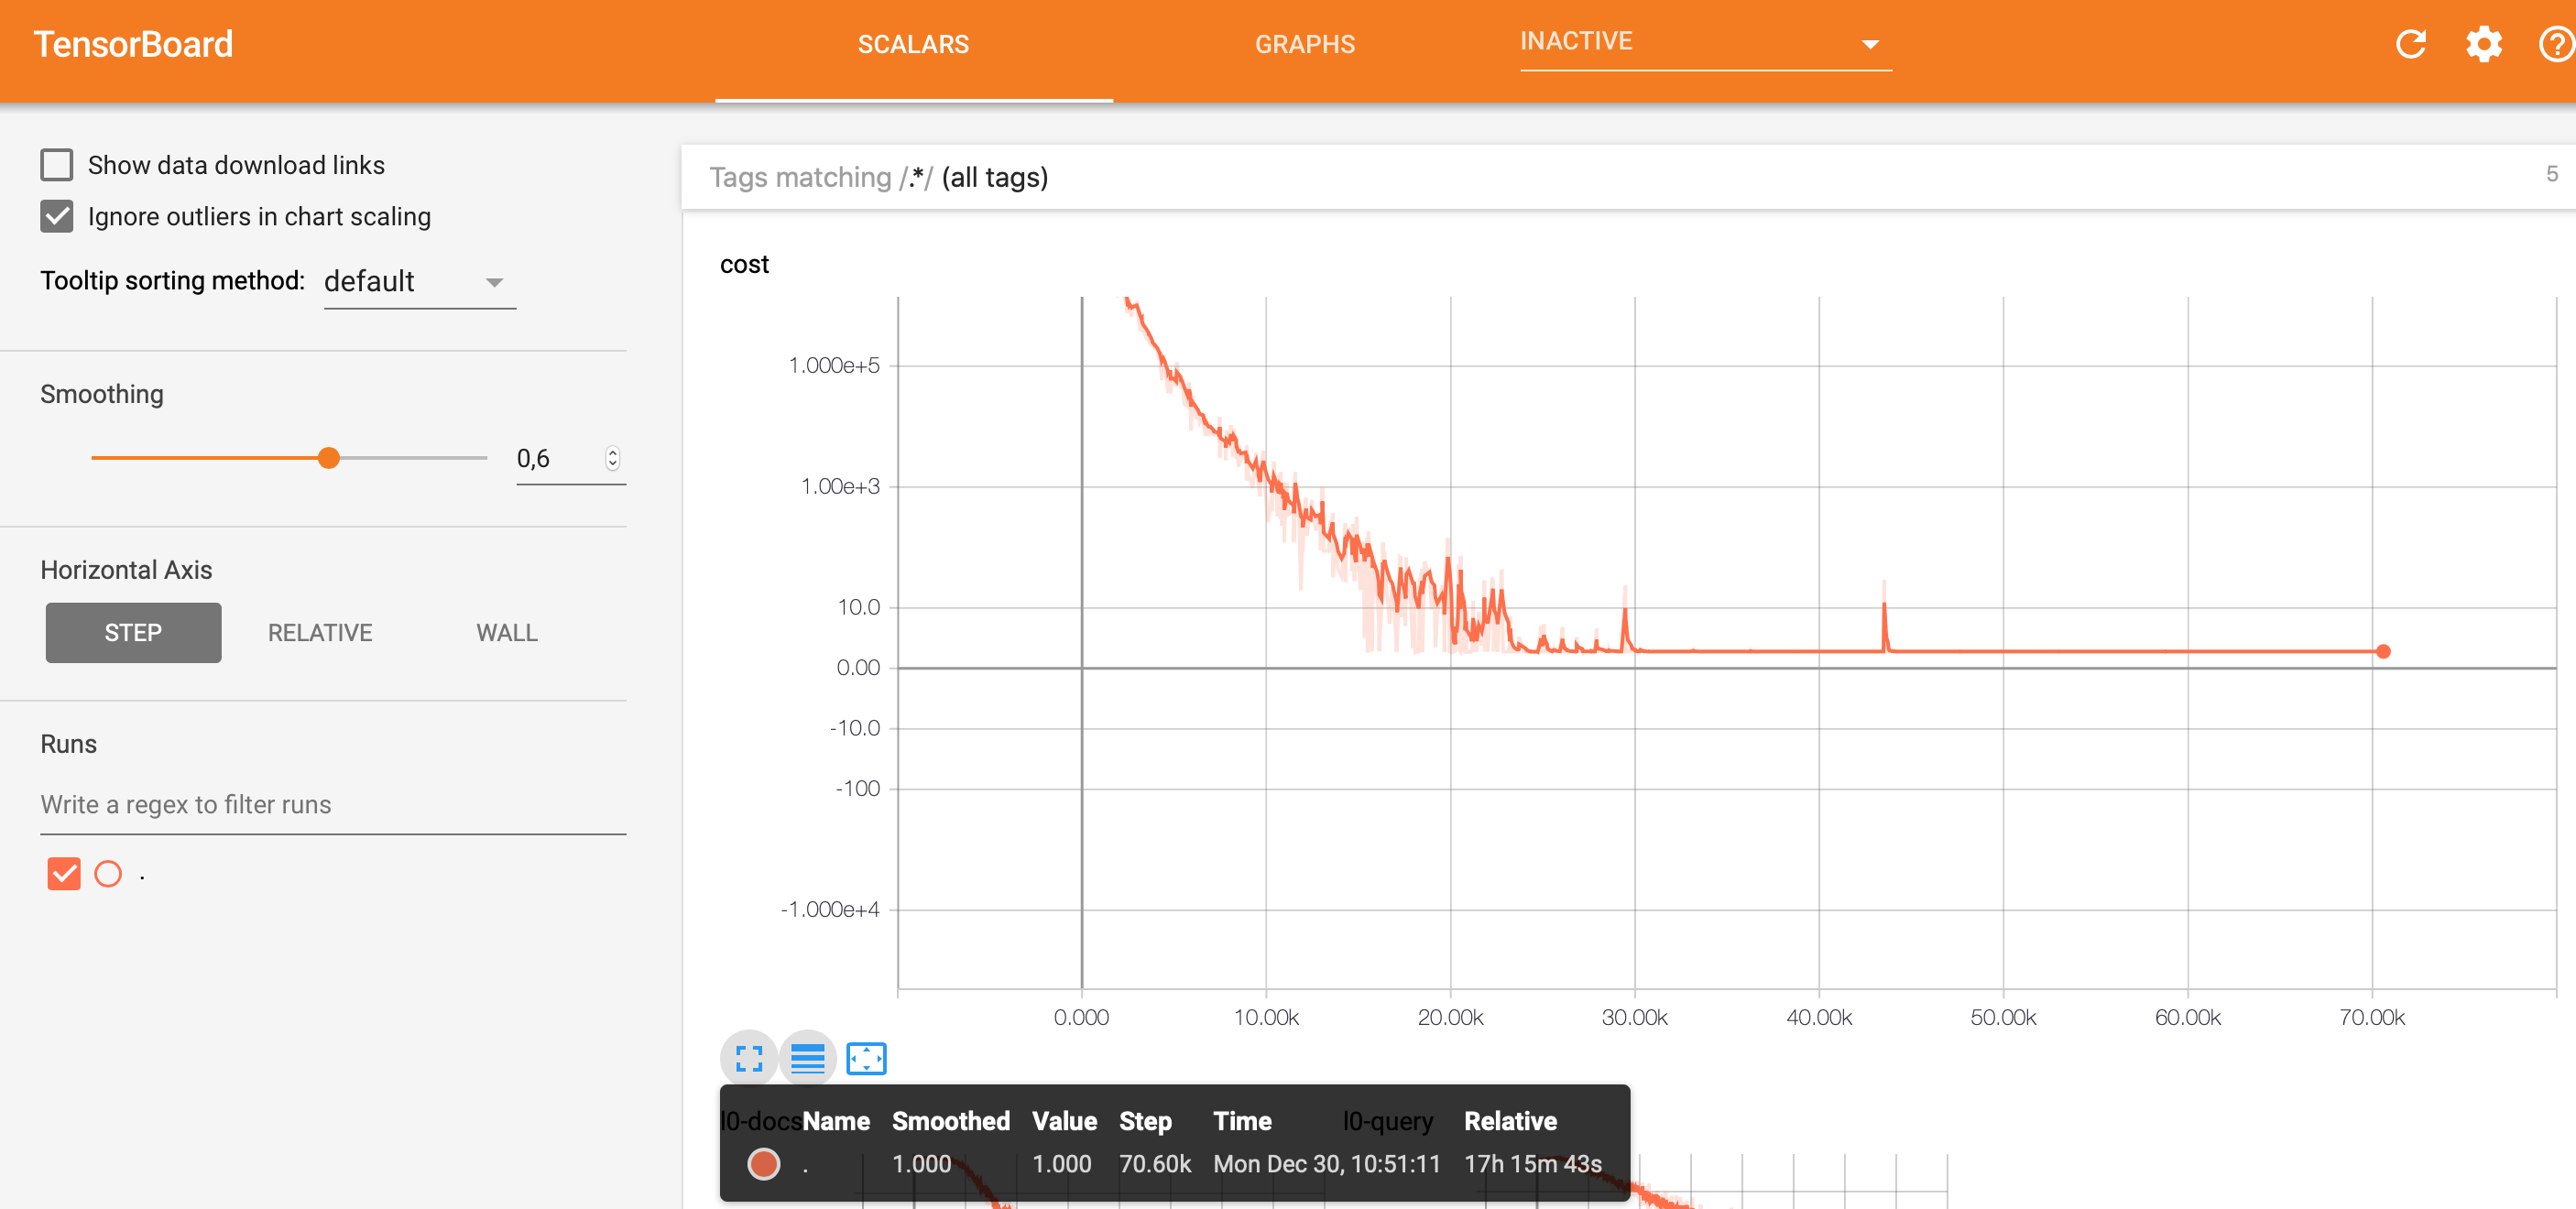
\includegraphics[trim=26.6cm 5cm 5cm 9cm,clip=true,width=0.96\textwidth]{Bildschirmfoto_2019-12-30_1.png}}
% Remove the [...] argument if the original caption should be used in the figure list.
\caption[Cost function swiveling in to a value of 3]{Cost function approaching zero, but swiveled in to a value of 3 after about 22,000 training steps and stayed there} 
\label{fig:2019-12-30:cost-fn} % \label has to be placed AFTER \caption (or \subcaption) to produce correct cross-references.
\end{figure}

After discussing the issue with the thesis advisor assistance, 
    a different document collection dataset (\verb|collection.air-subset.tsv|) 
    which is based on MS MARCO, but preprocessed for the Advanced Information Retrieval 
    lecture exercise, was chosen for experimentation.
This document collection should have a better ratio between relevant and non-relevant documents,
    than the previously utilized one.
\todo{@Sebastian: Sollen/Können wir das genauer beschreiben, wie das AIR collection.airsubset.tsv generiert wurde?}
For evaluation, as a query file, resp. qrels file the files \verb|queries.air-subset.tsv| resp.
    \verb|qrel.air-subset.tsv| were also downloaded from the university's OwnCloud server 
    \footnote{Advanced IR lecture exercise files (collection, query, qrel) \url{https://owncloud.tuwien.ac.at/index.php/s/1MugXnkP607Qm8P}}.
It was also tried to use as training dataset the MSMARCO \verb|triples.train.small.tsv| (27 GB)
    \footnote{MSMARCO passage ranking training set triples.train.small.tsv download link \url{https://msmarco.blob.core.windows.net/msmarcoranking/triples.train.small.tar.gz}}.
Due to Google Colab's hardware constraints of ca. free 30 GB disk space, rather than using the whole training,
    a smaller proportion of training triples (e.g. 6 GB) were used.

In another experiments, saving the model after every ten-thousand training steps, when training for about 70,000 steps, 
    showed, that, the longer the model had been trained, the more sparse the tensor representations became.
Either, the model was trained too long and the query representations had been the zero vector,
    or the query representation has non-zero values, however all documents are returned for such a query or 
    retrieval takes far too long to be feasible.
In other words, the IR systems either returns all documents from the collection as relevant or no document.
Obviously, the system was not able to learn and polarize different semantic concepts.

To better gauge SNRM during index construction and retrieval, Python logging was expanded,
    to log the sparsity of inferred query and document representations.
This showed useful to get a glimpse of how useful resulting representations are, and for deciding
    which models might not be worth for further experiments.
Especially for retrieval, besides sparsity, logging was also added for gaining knowledge of
    the number of existing documents per latent term dimension in the inverted index. \\
Tensorboard Logging was extended with diagrams of the number of zeros in tensors (sparsity) of 
    query and document representations, as well as the mean representations' values .
Aside from that, validation runs between model training phases, were separated from the Tensorboard logging 
    of training runs.

\subsubsection*{Variation and testing of different hyperparameters and configurations}
Experiments over multiple weeks were executed, trying to find a way to cope with the representations' sparsity 
    as the key problem.
Examination of the tests revealed, that the loss function approaches the value zero, 
    despite little variation, just after a few ten-thousand training steps.
The sparsity, the number of zeros, of the query and document representation tensors, similarly, 
    approaches soon 1, i.e. the representations coefficients tend to become all zero too fast.\\
Hyperparameter and the neural network architecture is configurable via the Python file \verb|"code/params.py"|.
In this configuration file, it is possible to easily adjust the number of neural network layers and neuron units
    for each layer separately, for instance.
Additionally, hyperparameters, like the learning rate, the convolution dropout rate, or SNRM's sparsity regulartization term
    are configurable.
Also, the maximum query and document length, which are used as the maximum length for trimming or padding tokenized text,
    are changeable using the config file.
Just to name a few modifications to SNRM's neural architecture during the test, the following number of layers and units per layer
    were attempted.
The labels "In" is the neural network input layer (embedding) and the number assigned is the number of neurons in this layer, 
    where "Out" is the output layer resp. query or document representation vector dimension.
The numbers between "In" and "Out" are the number of units per hidden layer. 
Hidden layers are separated by a dash ("-")
\begin{itemize}
    \item In: 300 -> 100 - 100 - 300 -> Out: 5000
    \item In: 300 -> 100 - 100 - 100 -> Out: 5000
    \item In: 300 -> 100 - 100 -> Out: 5000
    \item In: 300 -> 100 - 300 -> Out: 5000
    \item In: 300 -> 50 - 50 -> Out: 5000
\end{itemize}

Rather than using only an output dimension of 5,000, experiments were tried with 10,000 output neurons, too.
Unfortunately, the memory of the available local computers and on Google Colab was insufficient to create an inverted index
    with 10,000 dimensions.
Instead of using just a 100-dimensional GloVe embedding (\verb|"glove.6B.100d.txt"|), it was also tried to 
    use a 300-dimensional word vectors (\verb|"glove.42B.300d.txt"|).
Related to the chosen embedding, it was moreover tried to either set the embedding trainable or not.
For configuring the query and document max length, a Python script was written to identify statistics of the 
    number of tokens per query and document passages in the training set and in the document collection, 
    like the mean and several quantiles
With these statistics the max query and document length was varied in multiple experiments.

Concerning hyperparameters, several tests were run with either different convoluion dropout rates or no dropout, 
    the learning rate was varied, and also the regularization term $\lambda$.\\
Zamani et al. employed a regularization parameter $\lambda$
    in the loss function, that should control the sparsity of the model's output representations.
In their paper, the authors revealed in a diagram an association between the value of the regularization term $\lambda$ and the 
    sparsity as well as the information retrieval evaluation metric "Mean average precision" (MAP).
Interestingly, in the author's diagram the representations do not become too fast too sparse.
For example,  with a regularization term of $\lambda=1*10^{-7}$, their representation sparsity is at 100,000 training steps 
    just at about $0.7 - 0.8$. \cite{zamani:2018:from-neural-reranking-to-neural-ranking}\\
Varying the regularization term $\lambda$ in the authors' endorsed interval of $[1*10^{-7}, 5*10^{-9}]$ and 
    even trying non-destined values, like 0, 30, or 1,000, but also negative values, did not change the course 
    of the representations' sparsity significantly in Tensorboard.

The code in Listing~\ref{tensorflow-cost-function-calc} shows a piece of the original SNRM model's cost function calculation.
The cost function is basically composed of the hinge loss, a L1 regularization reduces the coefficients of queries and 
    tuples of positive and negative document passages, and additionally, the effect of the regularization is
    controlled by the \texttt{regularization\_term}.

\begin{lstlisting}[language=Python,frame=single,breaklines=true,float=tbh,caption=Cost function calculation in SNRM TensorFlow implementation,label=tensorflow-cost-function-calc]
# the hinge loss function for training
self.loss = tf.losses.hinge_loss(
                logits=logits, 
                labels=self.labels_pl, 
                scope='hinge_loss', 
                reduction=tf.losses.Reduction.MEAN)

# the l1 regularization for sparsity. Since we use ReLU as 
# the activation function, all the outputs of the
# network are non-negative and thus we do not need to get 
# the absolute value for computing the l1 loss.
self.l1_regularization = tf.reduce_mean(
    tf.reduce_sum(
        tf.concat(
            [self.q_repr, self.d1_repr, self.d2_repr], axis=1
        ), 
        axis=1),
    name='l1_regularization')

# the cost function including the hinge loss and the 
# l1 regularization.
self.cost = self.loss + 
    (tf.constant(self.regularization_term, dtype=tf.float32) * 
    self.l1_regularization)
\end{lstlisting}

Although, trying these stated different modifications to the neural network architecture, 
    embedding, hyperparameters, and other configuration values,
    the plots in Tensorboard still looked quite similar to previous experiments.
Figure~\ref{fig:2020-01-15:cost-fn-query-doc-repr-sparsity} shows plots of the 
    cost function and the representation sparsity of a query and document batch 
    for multiple training runs with different configurations.
The cost function was approaching the value 0 just after a few 10-thousand training steps.
Still, the query and document representations are getting too sparse too fast.
Especially, query representations tend to become more sparse earlier than document representations.
The latter is bad for retrieval, because no documents would be found for zero vector query representations, 
    despite having true positve coefficients in document representation vectors.
Therefore, the model training time was restricted due to the representations' rising sparsity,
    and as a result, the SNRM model could not deliver positive evaluation metrics.

% pictures of tensorboard diagramme 2020-01-15 Tensorboard snrm-extension.pdf
\begin{figure}[htbp]
\centering
\begin{subfigure}[b]{0.96\textwidth}
    \centering
    % trim: left bottom right top
    \frame{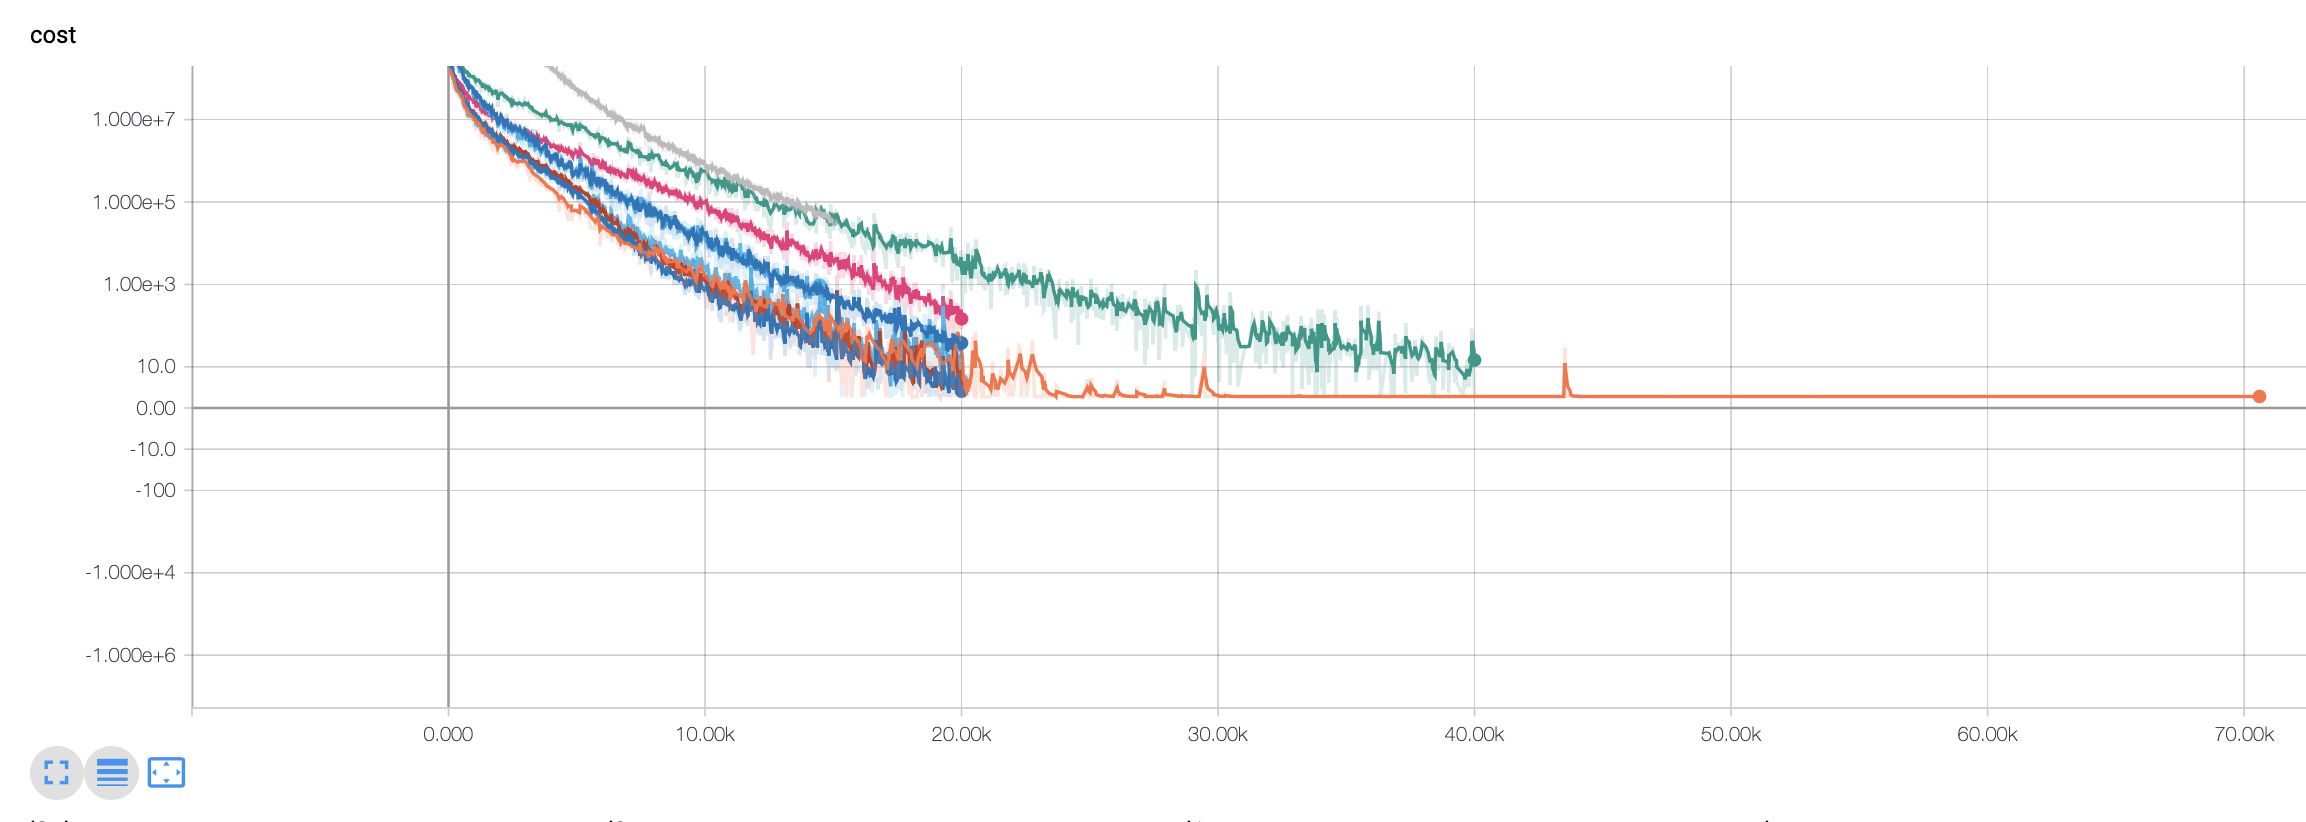
\includegraphics[trim=0.2cm 1cm 18.5cm 0cm,clip=true,width=\textwidth]{Bildschirmfoto_2020-01-15_1.png}}
    \subcaption{Cost function of multiple different runs approaching the value zero}
    \label{fig:2020-01-15:cost-fn}
\end{subfigure}
\begin{subfigure}[b]{0.45\textwidth}
    \centering
    \frame{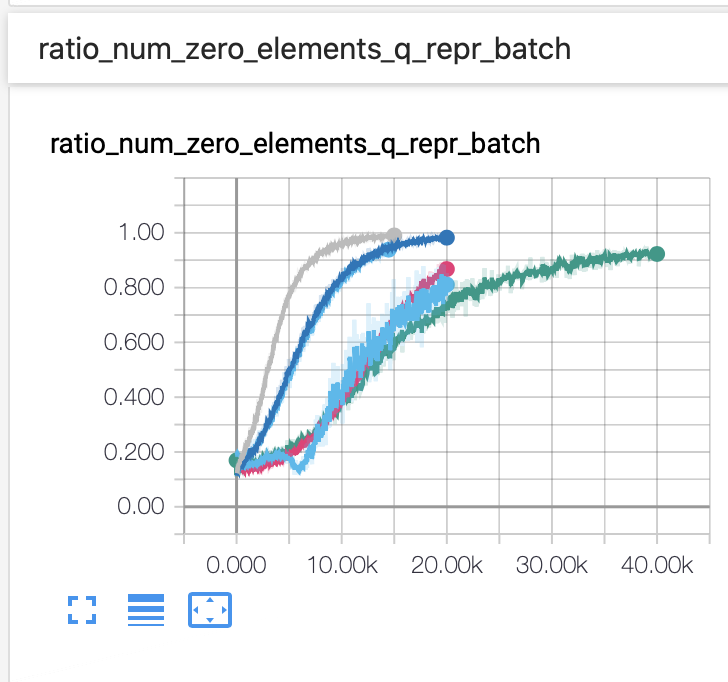
\includegraphics[trim=0.8cm 1.5cm 0cm 4cm,clip=true,width=\textwidth]{Bildschirmfoto_2020-01-15_2.png}}
    \subcaption{Course of representation sparsity as a function of training steps for query batches and different runs}
    \label{fig:2020-01-15:sparsity-query-repr}
\end{subfigure}
\hspace{0.042\textwidth}
\begin{subfigure}[b]{0.45\textwidth}
    \centering
    \frame{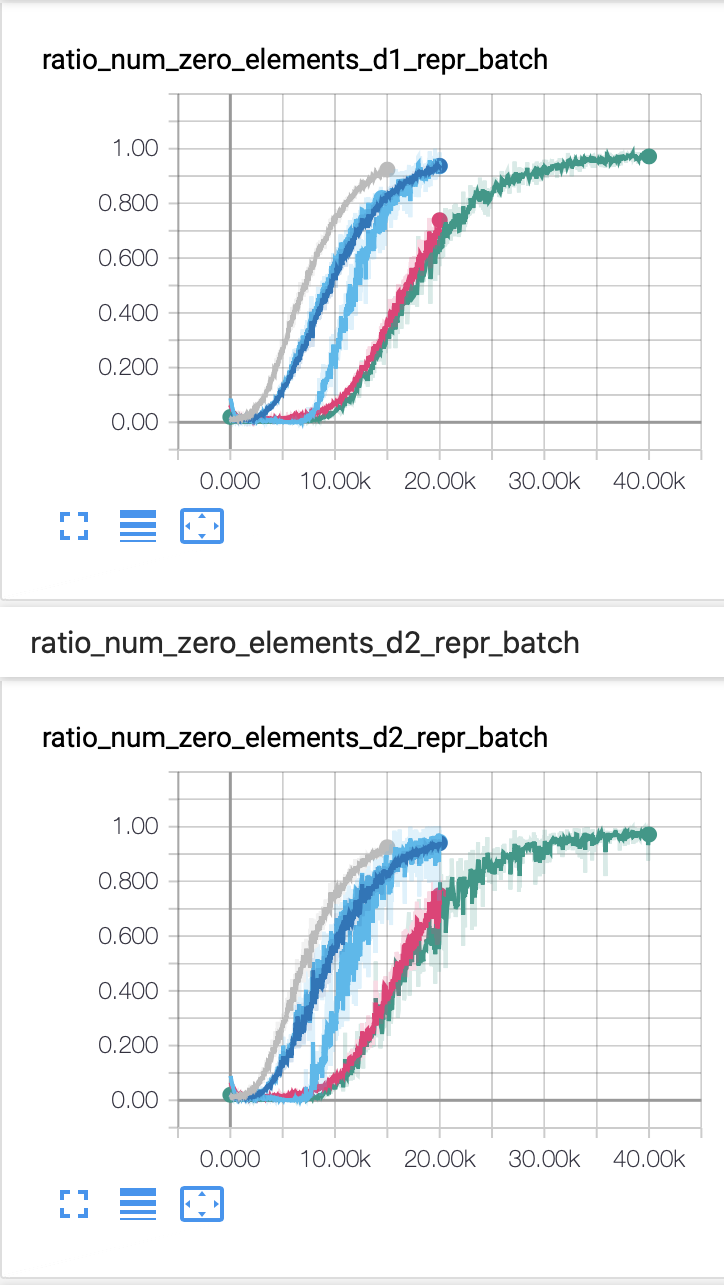
\includegraphics[trim=0.5cm 2cm 0cm 24.9cm,clip=true,width=\textwidth]{Bildschirmfoto_2020-01-15_3.png}}
    \subcaption{Course of representation sparsity as a function of training steps for document batches and different runs}
    \label{fig:2020-01-15:sparsity-doc-repr}
\end{subfigure}
% Remove the [...] argument if the original caption should be used in the figure list.
\caption[Costs function and course of representation sparsity for runs with different configurations and hyperparameters]{Cost function approaching 0 and representation sparsity of query and document batches nearing 1.0 after a few ten-thousand training steps for multiple training runs with different configurations and hyperparameter values}
\label{fig:2020-01-15:cost-fn-query-doc-repr-sparsity} % \label has to be placed AFTER \caption (or \subcaption) to produce correct cross-references.
\end{figure}

A further challenge was, that Google Colab terminated sessions regulary, probably based on time spent or usage.
The occurence of these timeouts, led to moving the index construction, retrieval and evaluation to the 
    local available personal computer, and using Google Colab only for training the model GPU-accelerated.
Further delays have happened, because sometimes Google refused the usage of a compute instance equipped with a GPU,
    and therefore enforcing the utilization of a non-GPU system, 
    or to wait until a GPU machine becomes available again.

\subsubsection*{Changing loss computation and neural network architecture}
In the original SNRM code the TensorFlow model was designed with two-dimensional convolution layers, 
    followed by a ReLu (Rectified Linear Unit) activation function.
The authors used ReLu to increase the sparsity of the tensors by the nature of ReLu,
    which maps negative values to zero.
If configured also a dropout could be added after the activation function.\\
Since it was already tried in vain to use only the hinge loss without any regularization as the 
    model's cost function, as a further attempt the model was modified additionally 
    to ommit the dropout and to use only a ReLu activation layer on the last layer, i.e. on the output.
That experiment leaded to a similar result regarding sparsity, albeit with more a bit more variation 
    in the cost function.
Figure~\ref{fig:2020-01-24:cost-fn-query-doc-repr-sparsity} shows TensorBoard diagrams of 
    the cost function and the representation sparsity of a query and document batch, where 
    the orange color represents training and in blue are validation steps.
In the plots, the cost function still swivels in at about the value 3, but oscillates more afterwards
    compared to previous experiments.
However, as the plot of the query and document representation sparsity show, the sparsity 
    progresses too fast to 1 after about 20,000 steps.
These plots originate from a model without any L1 regularization, that is its loss function equals 
    the hinge loss, and further, no dropout was used and the ReLu activation function was only applied 
    to the output convolution layer.

% image of 2020-01-24 tensorboard diagramme
\begin{figure}[htbp]
\centering
\begin{subfigure}[b]{0.96\textwidth}
    \centering
    % trim: left bottom right top
    \frame{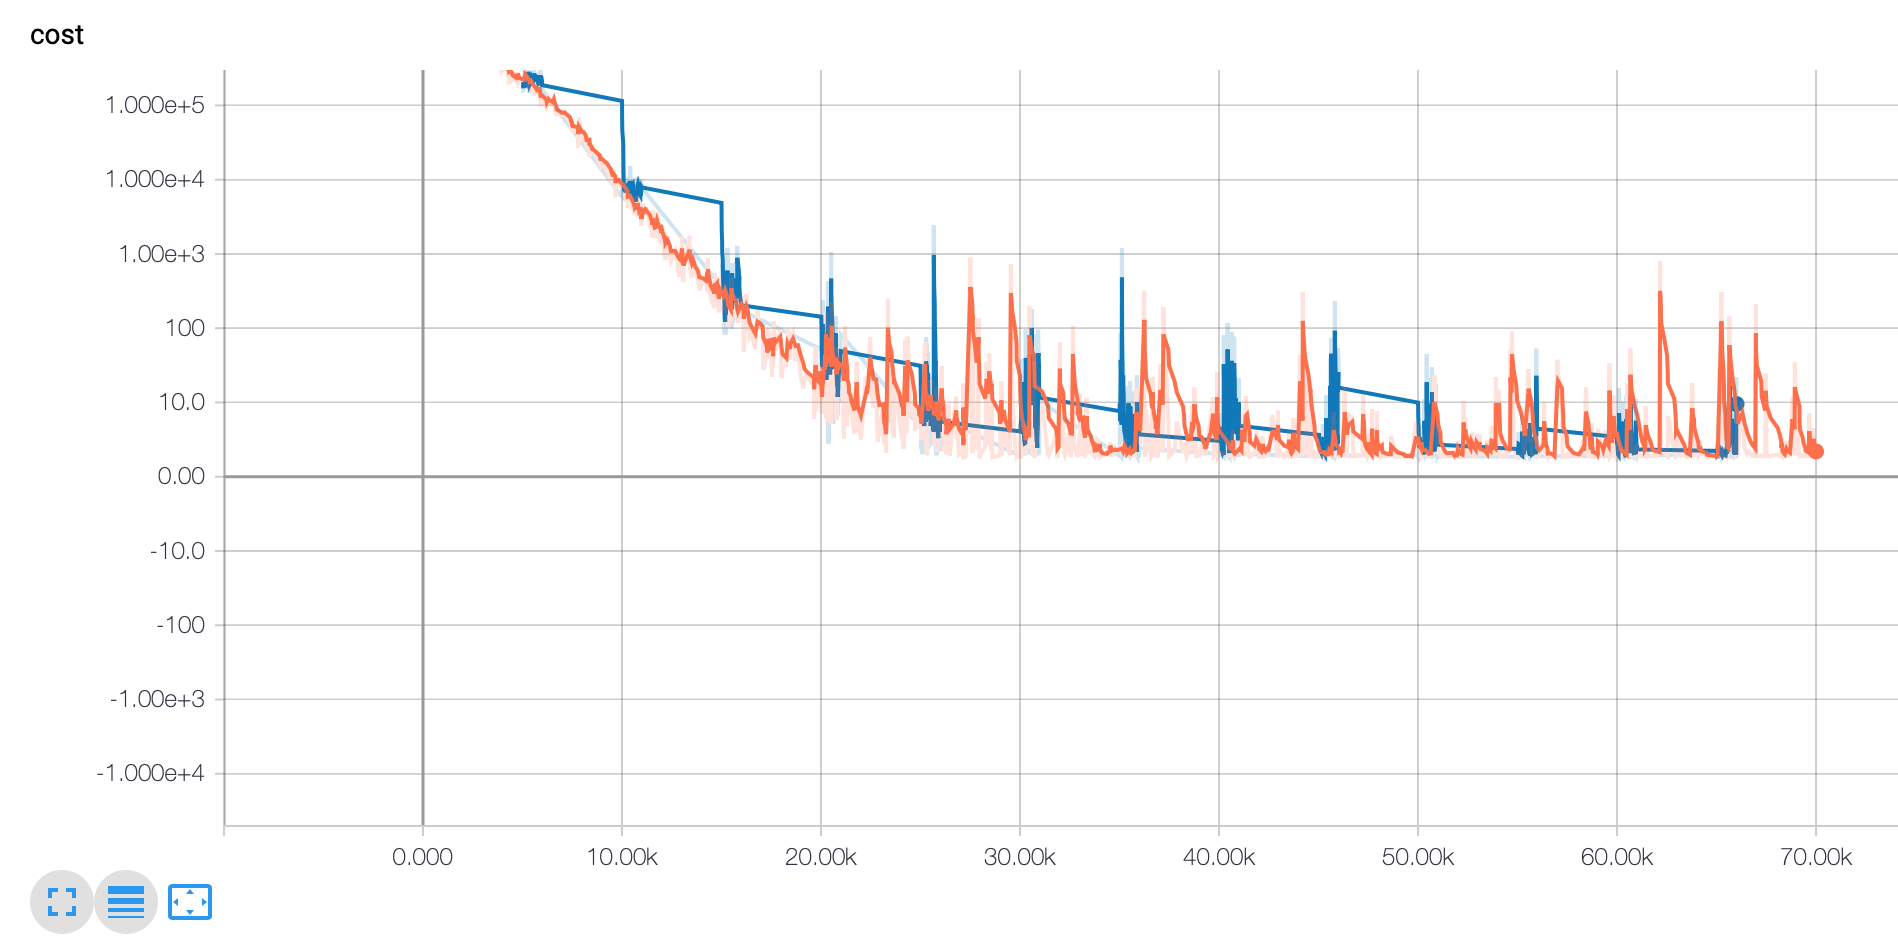
\includegraphics[trim=0.2cm 0cm 1cm 0cm,clip=true,width=\textwidth]{Bildschirmfoto_2020-01-24_1.png}}
    \subcaption{Cost function during training and validation approaching 0, but with oscillations}
    \label{fig:2020-01-24:cost-fn}
\end{subfigure}
\begin{subfigure}[b]{0.45\textwidth}
    \centering
    \frame{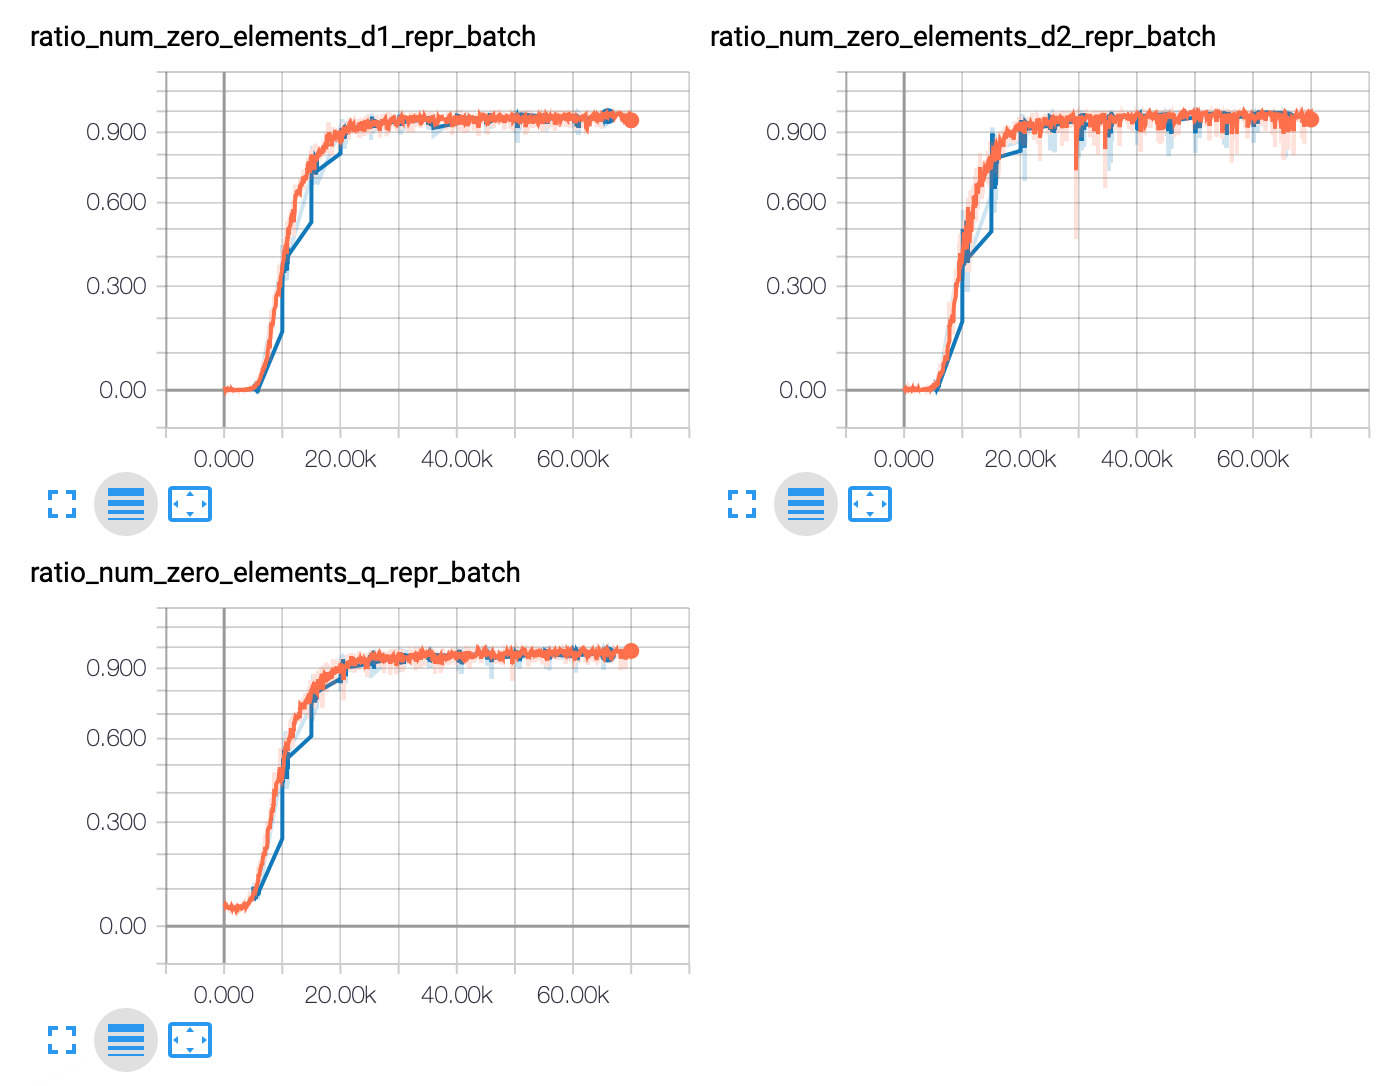
\includegraphics[trim=0.5cm 0cm 24cm 19cm,clip=true,width=\textwidth]{Bildschirmfoto_2020-01-24_2.png}}
    \subcaption{Course of representation sparsity as a function of steps for query batches during training and validation}
    \label{fig:2020-01-24:sparsity-query-repr}
\end{subfigure}
\hspace{0.042\textwidth}
\begin{subfigure}[b]{0.45\textwidth}
    \centering
    \frame{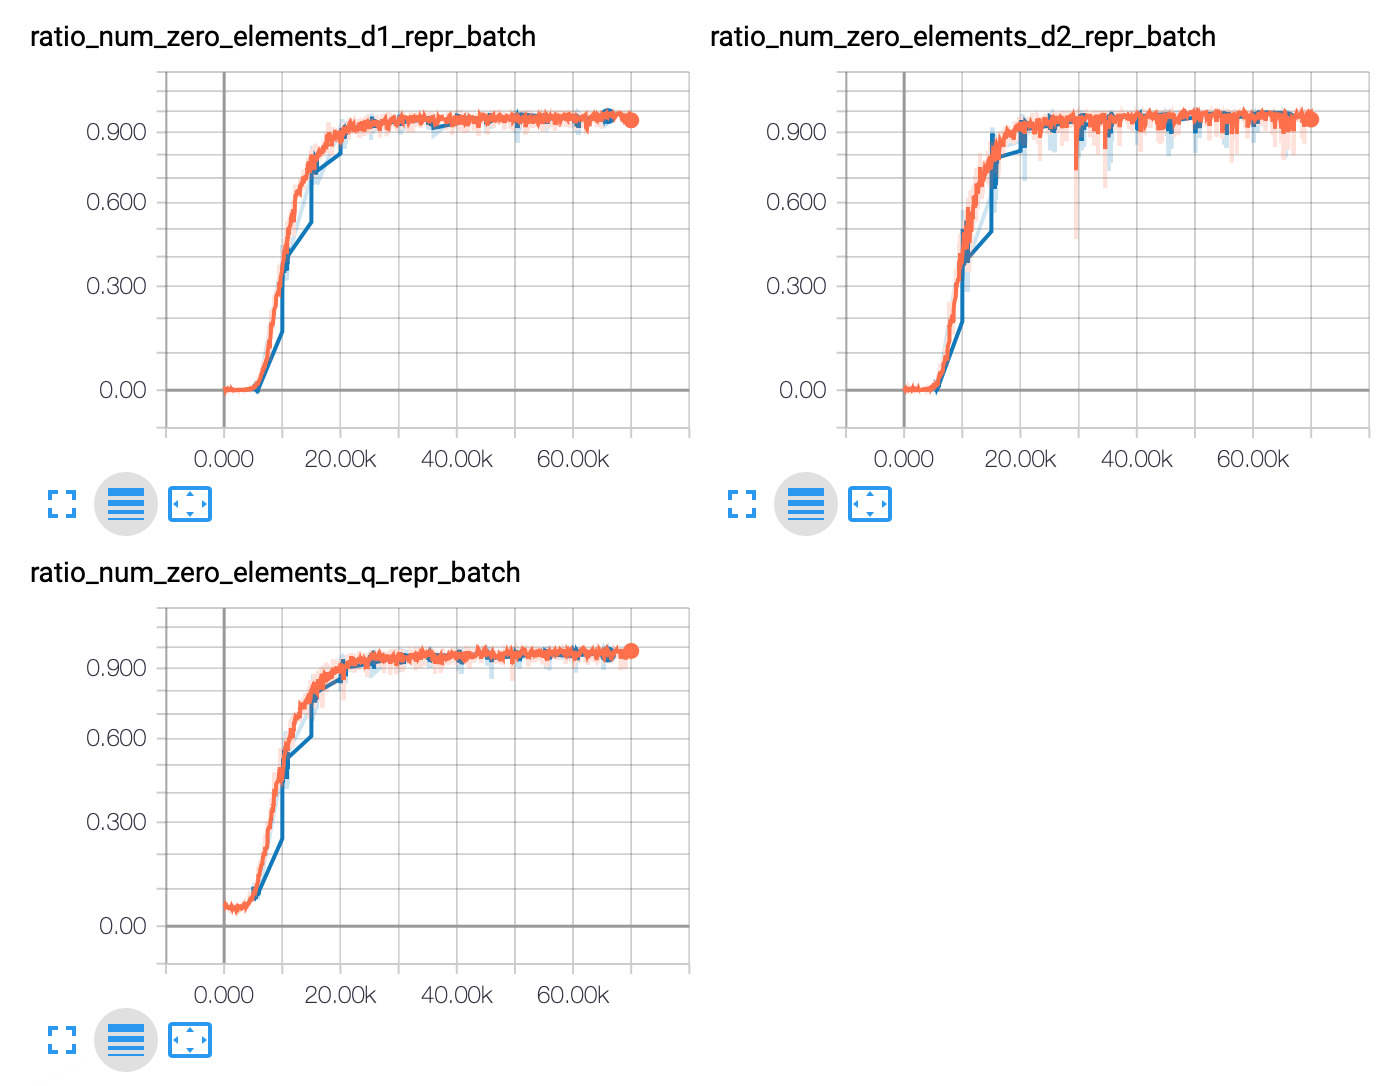
\includegraphics[trim=24.5cm 19cm 0cm 0cm,clip=true,width=\textwidth]{Bildschirmfoto_2020-01-24_2.png}}
    \subcaption{Course of representation sparsity as a function of steps for document batches during training and validation}
    \label{fig:2020-01-24:sparsity-doc-repr}
\end{subfigure}
% Remove the [...] argument if the original caption should be used in the figure list.
\caption[Costs function and representation sparsity for a run without L1 regularization, without dropout and ReLu only on the last layer]{Cost function approaching 0 and representation sparsity of query and document batches nearing 1.0 after about 20,000 training steps for a training (in orange) and validation (in blue) run with a model comprising as cost function no L1 regularization (i.e. only the hinge loss), no dropout and a ReLu activation function only on the last convolution layer}
\label{fig:2020-01-24:cost-fn-query-doc-repr-sparsity} % \label has to be placed AFTER \caption (or \subcaption) to produce correct cross-references.
\end{figure}

The model experiments and results have been discussed with the advisor assistance, subsequentially.
Another proposed try was to adjust the tensor operation on the logits for the hinge loss,
    while keeping the previous neural network design, with only one ReLu activation function at the output layer and
    without using dropout.
In the original SNRM code a hinge loss function is used between given truth labels
    (i.e. determining which document is more relevant to a given query),
    and logits.
Originally, the logits were computed as a tensor multiplication (\texttt{tf.multiply}) of 
    a positve and a negative representation's batch and a query representation's batch,
    followed by a sum computation (\texttt{tf.reduce\_sum}), 
    and a concatenation of the two tensors (\texttt{tf.concat}).
The code in Listing~\ref{tensorflow-logits-computation} shows part of the original SNRM source code for the 
    logits computation for the hinge loss.

\begin{lstlisting}[language=Python,frame=single,breaklines=true,float=tbh,caption=Logits computation for loss in SNRM TensorFlow implementation,label=tensorflow-logits-computation]
logits_d1 = tf.reduce_sum(
                    tf.multiply(self.q_repr,self.d1_repr),
                    axis=1, keep_dims=True)
logits_d2 = tf.reduce_sum(
                    tf.multiply(self.q_repr,self.d2_repr),
                    axis=1, keep_dims=True)
logits = tf.concat([logits_d1, logits_d2], axis=1)

# the hinge loss function for training
self.loss = tf.reduce_mean(tf.losses.hinge_loss(
                                        logits=logits, 
                                        labels=self.labels_pl, 
                                        scope='hinge_loss'))
\end{lstlisting}

In the course of this experiment, rather than using a sum reduction, it was tried to use
    a mean reduction (\texttt{tf.reduce\_mean}) instead for each document's logit computation.
Interestingly, without using a L1 regularization the representation sparsity had settled down after
    a few ten-thousand steps to about 0.8.
Compared to previous runs the sparsity approached 1.0 always, even without a L1 regularization utilized.
The cost function had started at not such a high values than before, but neared the value 1 much faster 
    and stays there.
Further experiments based on that were carried out, with the interest of adding a L1 regularization 
    and testing the controllability of the sparsity with the regularization term parameter $\lambda$.
Surprisingly, it was possible to change the query and documentation sparsity during training runs
    with different values for $\lambda$.
It was possible to increase the sparsity to a quite constant and desirable value of approx. 0.9.
When compared to previous attempts, the sparsity had not been controllable.
In Figure~\ref{fig:2020-02-07:relu-only-last:cost-fn-query-doc-repr-sparsity} 
    the cost function and the representation sparsity as a function of training steps is shown
    for multiple runs with different regularization term $\lambda$ values
    and where the hinge loss' logits computation comprisses mean reduction instead of sum reduction
    of a model with the ReLu activation function only on the output layer.

%  images of 2020-02-07 tensorboard diagramme.pdf
\begin{figure}[htbp]
\centering
\begin{subfigure}[b]{0.96\textwidth}
    \centering
    % trim: left bottom right top
    \frame{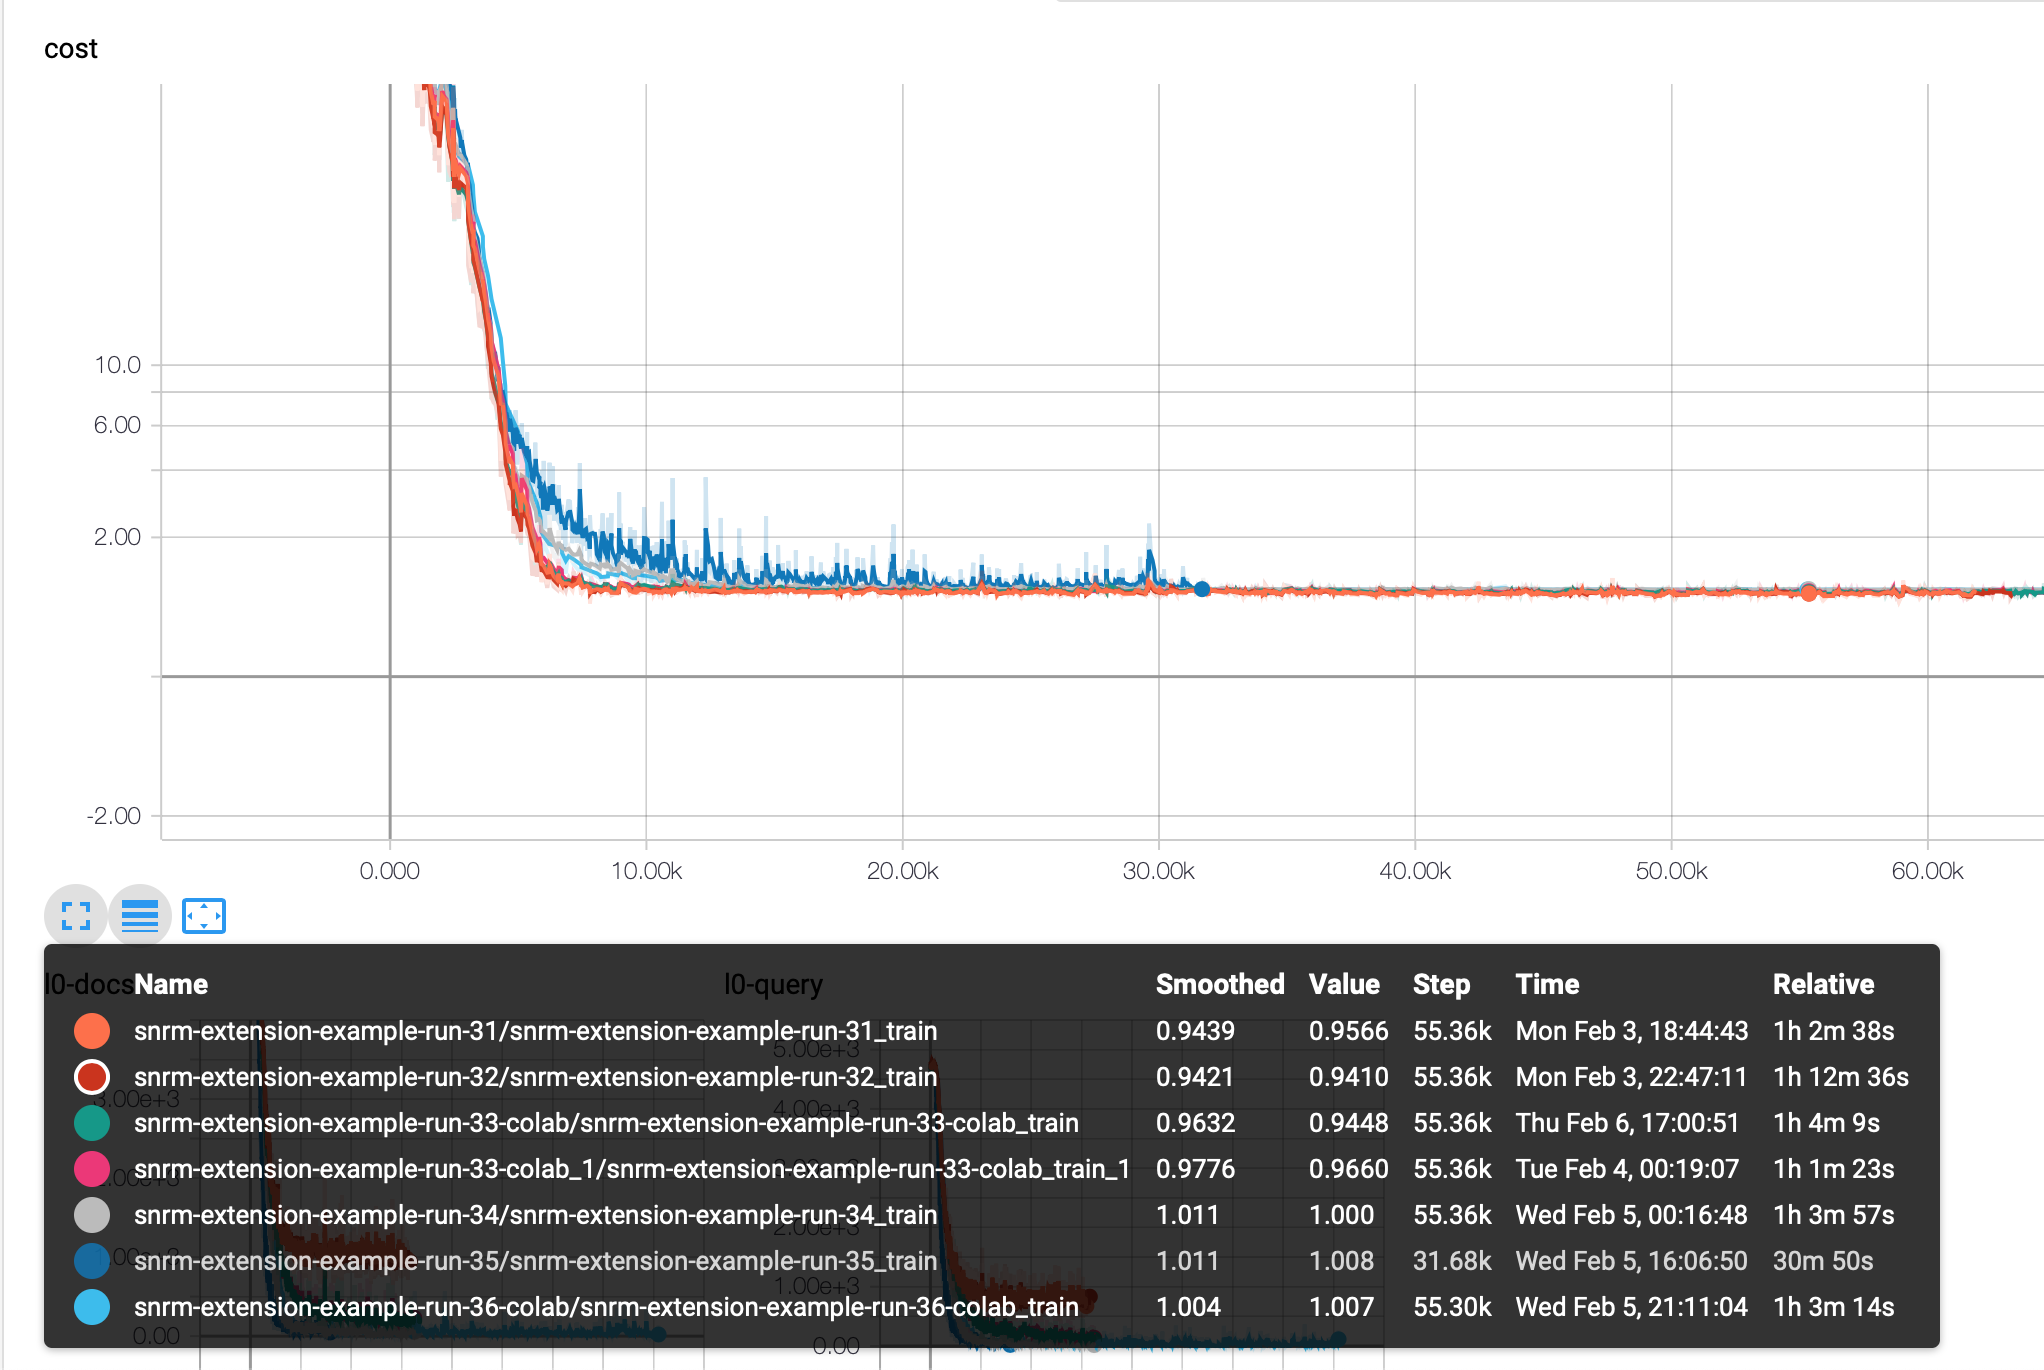
\includegraphics[trim=0.2cm 15cm 2cm 0.2cm,clip=true,width=\textwidth]{Bildschirmfoto_2020-02-07_relu-only-last_1.png}}
    \subcaption{Cost function of multiple runs with different regularization term $\lambda$ values}
    \label{fig:2020-02-07:relu-only-last:cost-fn}
\end{subfigure}
\begin{subfigure}[b]{0.45\textwidth}
    \centering
    \frame{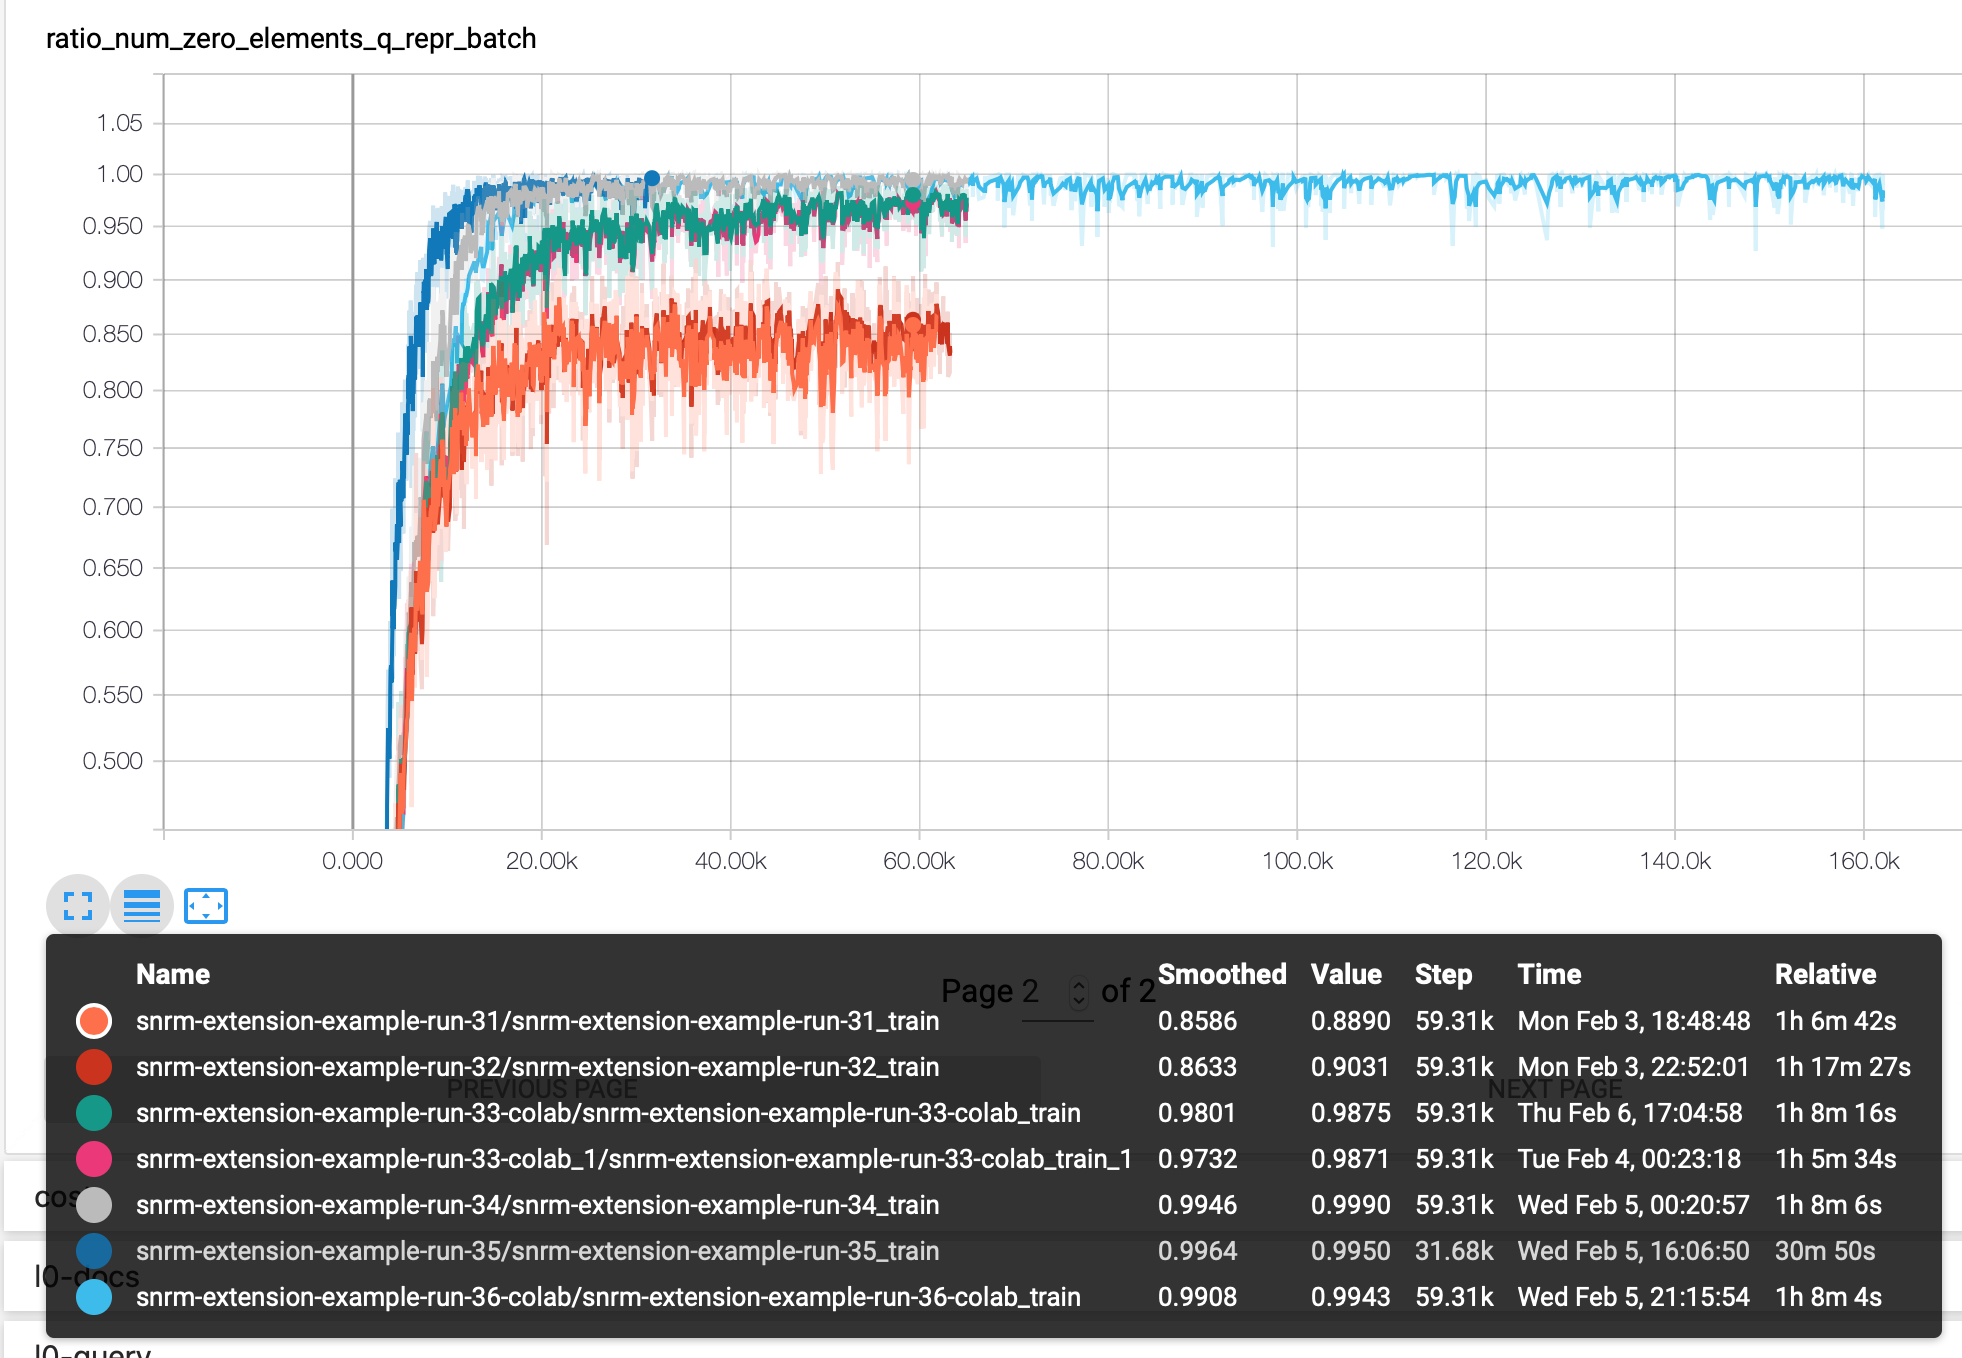
\includegraphics[trim=0.5cm 15cm 32cm 0.2cm,clip=true,width=\textwidth]{Bildschirmfoto_2020-02-07_relu-only-last_3.png}}
    \subcaption{Multiple runs with different regularization term $\lambda$ values show a controllable course of representation sparsity for query batches}
    \label{fig:2020-02-07:relu-only-last:sparsity-query-repr}
\end{subfigure}
\hspace{0.042\textwidth}
\begin{subfigure}[b]{0.45\textwidth}
    \centering
    \frame{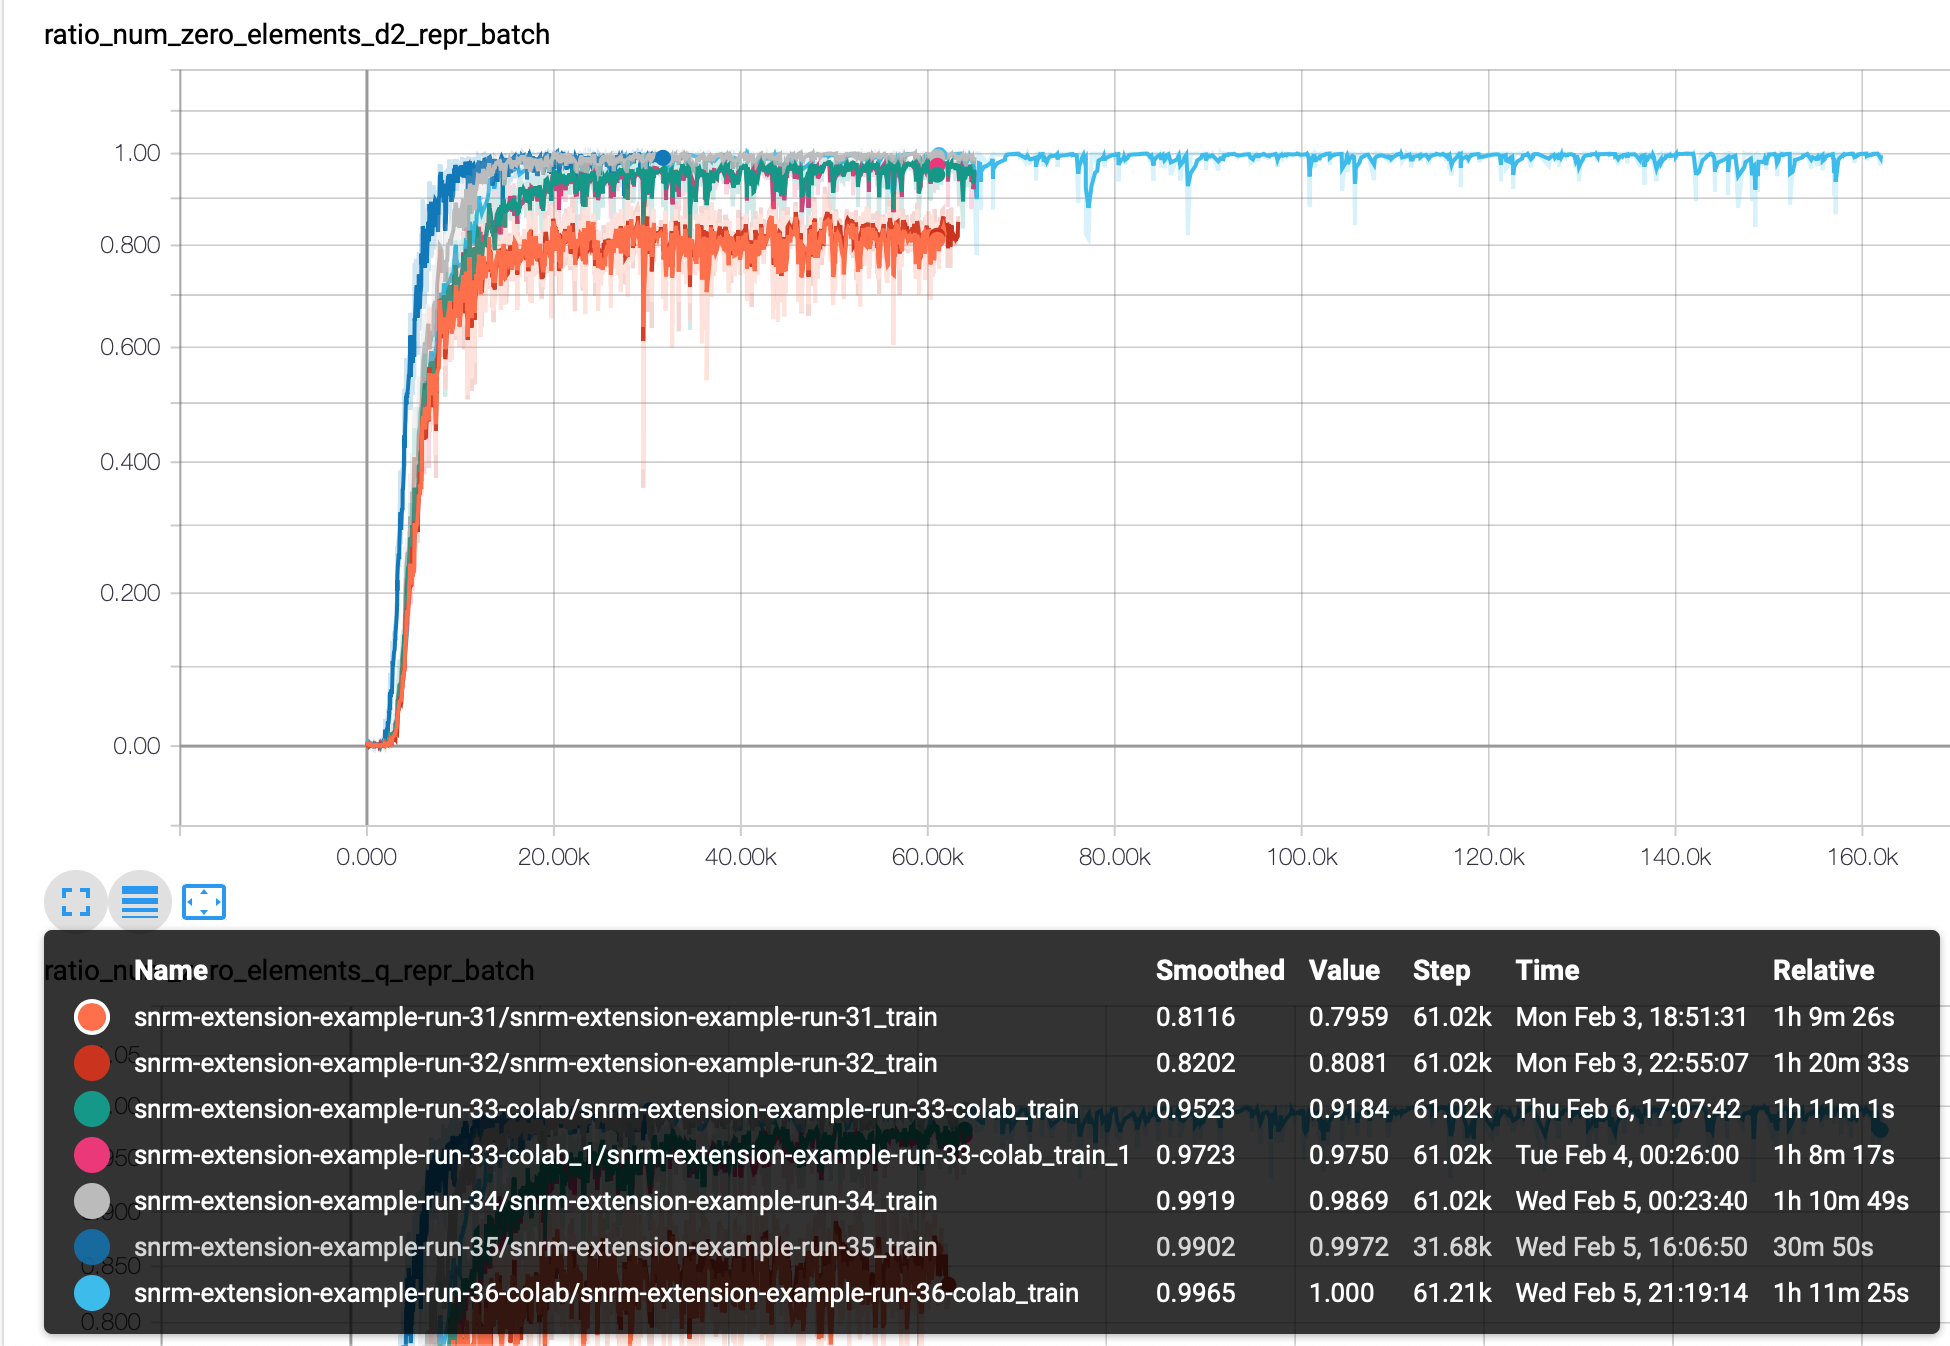
\includegraphics[trim=0.5cm 14.7cm 31cm 0cm,clip=true,width=\textwidth]{Bildschirmfoto_2020-02-07_relu-only-last_2.png}}
    \subcaption{Multiple runs with different regularization term $\lambda$ values show a controllable course of sparsity for document batches}
    \label{fig:2020-02-07:relu-only-last:sparsity-doc-repr}
\end{subfigure}
% Remove the [...] argument if the original caption should be used in the figure list.
\caption[Costs function and controllable sparsity of multiple runs with different values of regularization term $\lambda$ of a model comprising sum reduction for hinge loss' logits computation, no dropout and ReLu only after the last layer]{Cost function approaching approx. 1.5 and controllable representation sparsity of query and document batches for multiple runs with different regularization term $\lambda$ values of a model comprising no dropout, mean reduction instead of sum reduction for the hinge loss' logit computation and a ReLu activation function only after the last convolution layer}
\label{fig:2020-02-07:relu-only-last:cost-fn-query-doc-repr-sparsity} % \label has to be placed AFTER \caption (or \subcaption) to produce correct cross-references.
\end{figure}

Additionally, it was tried to add the ReLu activation function again for all layers, instead of 
    only for the last one, for this experiment design, but that leaded to even larger, undesired 
    differences in sparsity between document and query representations.
Therefore, the Relu activation function was only utilized after the last convolution layer for the
    subsequent experiments.
In Figure~\ref{fig:2020-02-07:relu-all:query-doc-repr-sparsity} the query and document representation
    sparsity is shown as a comparison for a model with ReLu activation functions 
    after all convolution layers, rather than only after the last convolution layer.

% image of sparsity difference for relu-all 2020-02-07 tensorboard diagramme relu all.pdf
\begin{figure}[htbp]
\centering
% trim: left bottom right top
\begin{subfigure}[b]{0.45\textwidth}
    \centering
    \frame{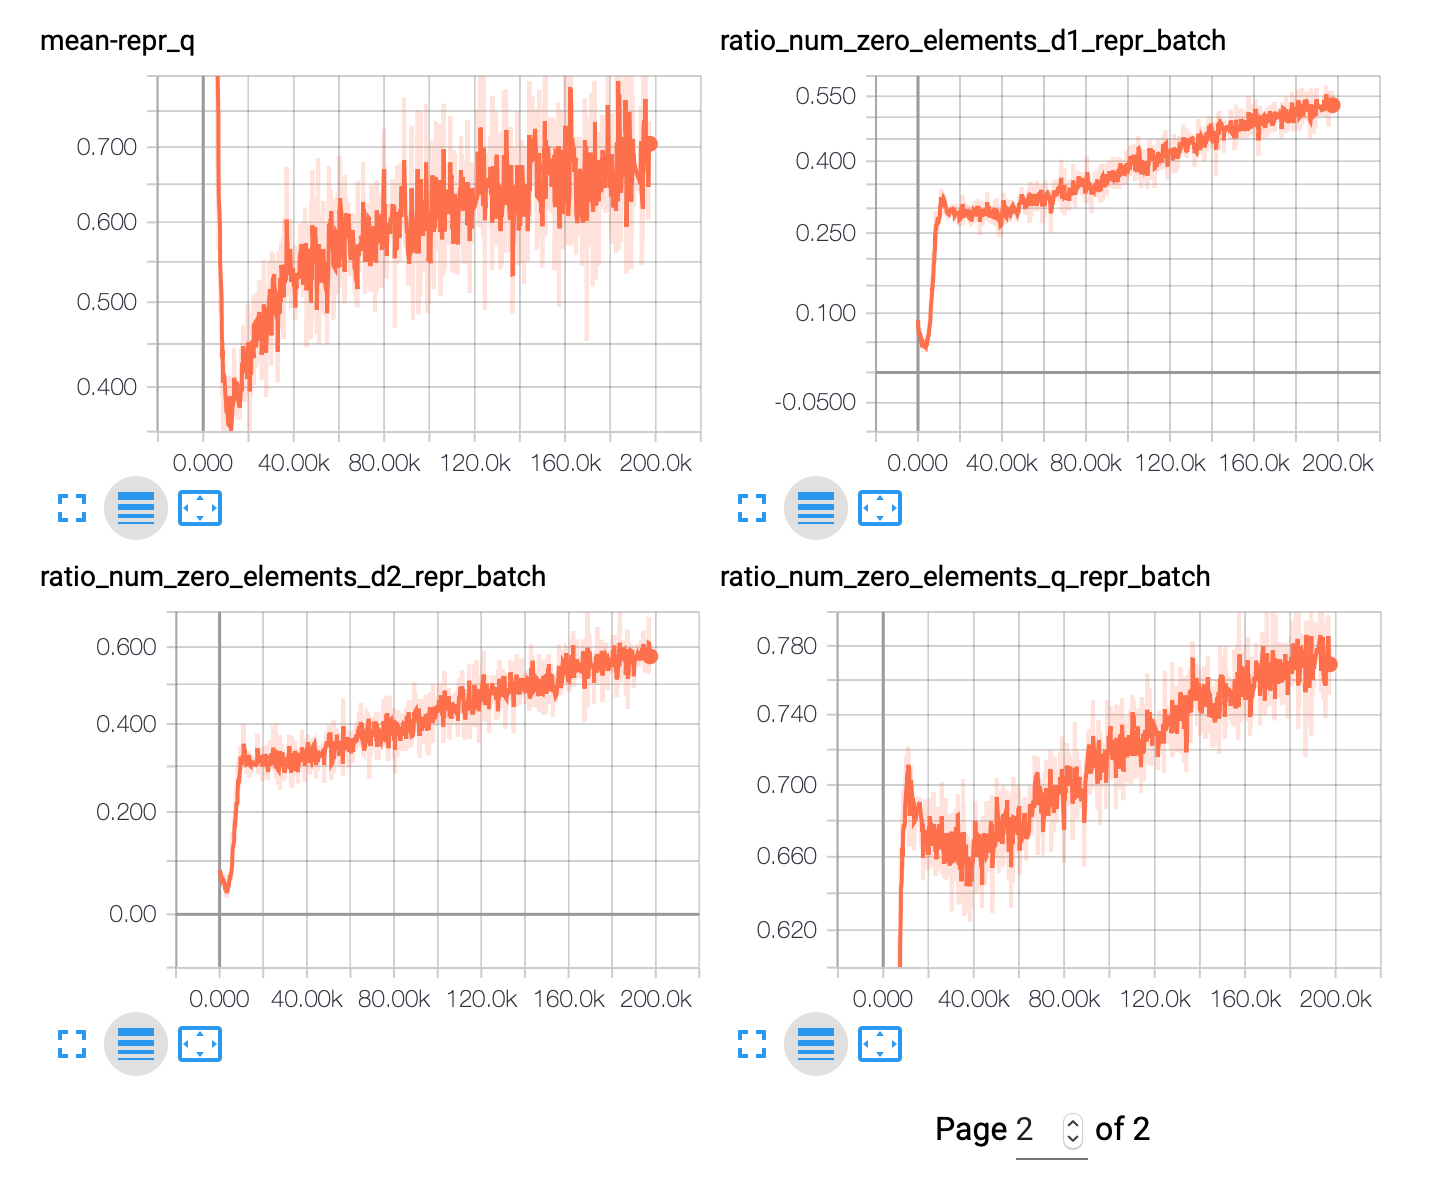
\includegraphics[trim=24.8cm 3.8cm 1.5cm 19.5cm,clip=true,width=\textwidth]{Bildschirmfoto_2020-02-07_relu-all_1.png}}
    \subcaption{Course of representation sparsity reaching about 0.76 at 200,000 steps for query batches}
    \label{fig:2020-02-07:relu-all:sparsity-query-repr}
\end{subfigure}
\hspace{0.042\textwidth}
\begin{subfigure}[b]{0.45\textwidth}
    \centering
    \frame{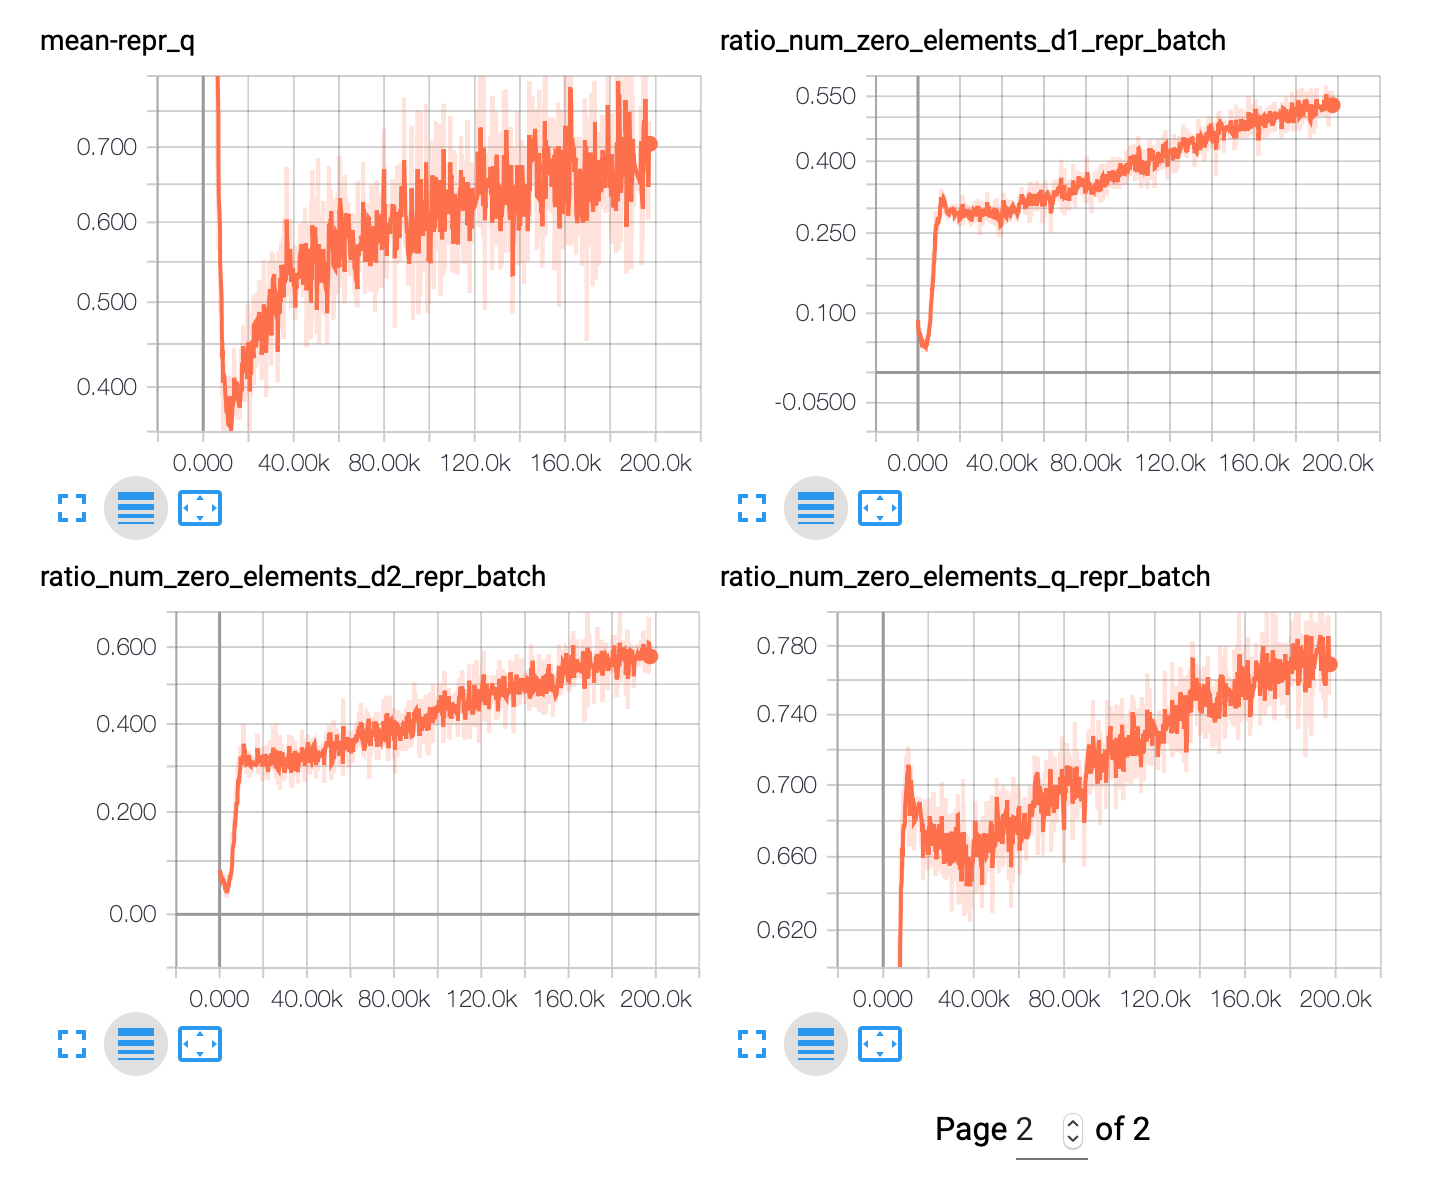
\includegraphics[trim=24.8cm 22.7cm 1.5cm 0.5cm,clip=true,width=\textwidth]{Bildschirmfoto_2020-02-07_relu-all_1.png}}
    \subcaption{Course of representation sparsity reaching about 0.50 at 200,000 steps for document batches}
    \label{fig:2020-02-07:relu-all:sparsity-doc-repr}
\end{subfigure}
% Remove the [...] argument if the original caption should be used in the figure list.
\caption[Query and document batches' representation sparsity of a model comprising sum reduction for hinge loss' logits computation, no dropout and ReLu after all convolution layers]{Quite different representation sparsity for query and document batches of a model comprising no dropout, mean reduction instead of sum reduction for the hinge loss' logit computation and ReLu activation functions after all convolution layers}
\label{fig:2020-02-07:relu-all:query-doc-repr-sparsity} % \label has to be placed AFTER \caption (or \subcaption) to produce correct cross-references.
\end{figure}

To illustrate the results of one of the training runs, where the sparsity was controllable, 
    here are a few document and query representation statistics for a model that has been 
    trained 60,000 steps, followed by an inverted index construction.
A Python script (\texttt{code/index\_stats.py}) was written to aggregate these document and
    query statistics.
The inverted index was created with 806,976 distinct document passages.
When analysing the document representations' dimensions, that is their latent term dimensions,
    there were at minimum 2,444 and at maximum 806,975 documents assigned for a latent dimension.
The latent dimensions' number of documents mean was 17,301.6318, the median was 3,660, and the
    0.75-quantile was 4,269.25, resp. the 0.90-quantile was 5,568.2.
Unfavorably, the sparsity of the document representations is bad for retrieval, because
    the number of documents for a certain latent term dimension is quite large.
For example, for one latent term dimension all indexed documents (806,976) are classified as relevant,
    and on average 17,301.6318 documents for a single out of 5,000 latent term dimensions
    would be returned for that model.\\
Concerning an analysis of the SNRM model's query representation statistics,
    the following metrics where gathered during inference of query representation tensors
    using the query file \texttt{queries.air-subset.tsv}.
The queries' mean of the non-zero value ratio was 0.00721, with a standard deviation of
    0.02364.
That is, the mean query representation sparsity was 99,279\%.
Over all query representations' minimum values the minimum was 0, and over all
    maximum values the maximum was 993.35760.
Finally, the mean value across all query representations' mean values was 0.20925, 
    resp. the standard deviation over all mean values was 0.08913.
Obviously, the maximum query representations' maximum value of 993.35760 lies far away from the mean of
    all vector mean values of 0.20925.
Summarized, the document representation sparsity is for this model still too low, because 
    too many document would be classified relevant, and the query representations' sparsity might be too big.

These results have concluded the experimentations regarding the SNRM model with extensions and modifications
    for running it with the MSMARCO passage ranking dataset.
The next steps in the practical part of the thesis was the migration of SNRM to PyTorch.

%%%%%%%%%%%%%%%%%%%%%%%%%%%%%%%%%%%%%%%%%%%%%%%%%%%%%%%%%%%%%%%%%%%%%%%%%%%%%%
\section{SNRM migration to PyTorch}

In this section the realization of the migration from the SNRM TensorFlow implementation to the PyTorch library
    is documented.
Additionally, observations and results of experiments are depicted, and
    challenges that have arisen and their respective attempts to solve them are presented.
This practical part of the thesis was done after setting-up the original SNRM application,
    and modifying it, to be runnable with the MSMRACO passage ranking dataset.

\subsection{Project setup and creation of Google Colab notebook}
For migration of the SNRM code to PyTorch, a new Git branch (\texttt{extension-pytorch})
    was created based on the previous SNRM extension code (\texttt{extension} branch), 
    i.e. previous modifications were partly reused for SNRM with PyTorch.
One of the first steps before moving on was to gain basic knowledge of PyTorch and AllenNLP
    and to take a few practical exercises and tutorials.
Especially, the programming API and the way neural models are defined is considerable
    different between PyTorch 1.4 and TensorFlow 1.4.

A new and clean Conda environment for the SNRM PyTorch project was set-up,
    without any installed pip or Conda software packets.
Just like before, the Google Colab platform was used and hence, previously 
    installed NVIDIA CUDA and cuDNN packages were uninstalled,
    and compatible versions for PyTorch were installed.
To be able to use GPU-accelerated model training, NVIDIA CUDA version 10.1.243-1 
    and NVIDIA cuDNN v7.6.4 were installed in Google Colab manually.
NVIDIA CUDA was downloaded from NVIDIA's CUDA Toolkit Archive
    \footnote{NVIDIA Developer CUDA Toolkit Archive website \url{https://developer.nvidia.com/cuda-toolkit-archive}}
    for Google Colab's operating system, currently at the time Ubuntu 18.04.3 LTS.
For downloading NVIDIA cuDNN a NVIDIA Developer Program Membership is required to be able to
    download the software from NVIDIA's cuDNN Archive
    \footnote{NVIDIA Developer cuDNN Archive website \url{https://developer.nvidia.com/rdp/cudnn-archive}}.
Subsequently, the packages according to Listing~\ref{installed-conda-pip-packages-colab-pytorch} 
    were installed using Conda and pip on the local system and in the Google Colab Notebook.
Implicitely, the NumPy package (version 1.18.1) and other dependent packages were downloaded
    and installed automatically by these package managers.

\begin{lstlisting}[language=bash,frame=single,breaklines=true,float=tbh,caption=Installed Conda and pip packages in Google Colab Notebook for SNRM PyTorch implementation,label=installed-conda-pip-packages-colab-pytorch]
conda install -qy -c pytorch pytorch=1.4.0 torchvision=0.5.0 \
                           cudatoolkit=10.1.243 python=3.7.6
pip install allennlp==0.9.0 tensorboard==2.1.0
\end{lstlisting}

After installing the necessary and at that time current packages, the migration of the actual source code
    was started.

\subsection{Adding application logging and migrating the configuration}

Unlike the original SNRM source code, a logger with an application-wide logging 
    configuration was setup (\texttt{code/app\_logger.py}),
    that not only writes log output to the console, but also to a rotating log file.
An advantage of the application logger was to more easily trace the the application behaviour,
    particularly regarding sparsity progression, a more centralized ability for configuring logging,
    and to overcome some consoles' maximum log line limitations.

Originally in the SNRM code, hyperparameters and more general configuration values were defined using
    TensorFlow's flags implementation \texttt{tf.flags}.
For instance, a \texttt{float} value for the parameter "learning rate" was configured and read with an 
    invokation of the code from Listing~\ref{flags-api-tensorflow} in the TensorFlow implementation.

\begin{lstlisting}[language=Python,frame=single,breaklines=true,float=tbh,caption=Example definition of a parameter “learning\_rate” using TensorFlow's flag api,label=flags-api-tensorflow]
import tensorflow as tf

# define value and description for parameter "learning_rate":
tf.flags.DEFINE_float('learning_rate', 
                      0.0001, 
                      'Learning rate for Adam Optimizer')
FLAGS = tf.flags.FLAGS
FLAGS._parse_flags()

# read and use parameter learning rate:
learning_rate=FLAGS.learning_rate
\end{lstlisting}

Several of the examined PyTorch projects, did not use anything similar to TensorFlow's
    \texttt{tf.flags} api.
Hence, the configuration capability was redesigned for the SNRM PyTorch version,
    to allow parameter configuration in a JSON file (\texttt{config/config.json}),
    and a configuration Python class (\texttt{code/config.py}) simplifies
    reading and accessing the configuration.

\subsection{Re-engineer data loading and processing}
In the Tensorflow SNRM extension project, standard Python functions were used 
    to open, read, parse and process data from several files, 
    like tokens, word embeddings, training triples, document collection 
    and query files.
Instead of reusing this code in the SNRM PyTorch project, functions from the
    AllenNLP library were used, e.g. to load and init a vocabulary from the token file,
    to initialize word embeddings from the embedding file,
    and to generate data batches automatically incl. padding or truncation 
    to an appropriate max length per batch for efficiency.
Reusability, efficiency, and a simpler more concise code overall justify the usage of the 
    AllenNLP library for these tasks, compared to implementing code once again by hand.
As a side effect the previously used dictionary Python class (\texttt{code/dictionary.py}) was not
    required anymore, due to the use of AllenNLP functions instead.
In order to be able to hand over structured data to AllenNLP functions for further processing, 
    two Python classes were added (\texttt{IrTripleDatasetReader}, \texttt{IrTupleDatasetReader})
    in the file \texttt{"/code/data\_loading.py"}, that implement AllenNLP's \texttt{DatasetReader}.
As the name of the interface suggests, these classes are responsible for reading tab separated files (tsv),
    and return those parsed, tokenized and filtered contents as fields within an AllenNLP \texttt{Instance} class.
Word tokenization resp. stopword filtering is also done using provided AllenNLP classes, 
    like \texttt{WordTokenizer}, \texttt{StopwordFilter}, and \texttt{JustSpacesWordSplitter} from the
    \texttt{allennlp.data.tokenizers} Python module.
The first one of the implemented data loaders, is in charge of reading input lines from training and validation
    triples files, with a format of \verb|"<query_string>\t<pos_doc_string>\t<neg_doc_string>"|.
And the other one, reads files with a format of \verb|"<id_string>\t<text_string>"|, and is used for
    reading entries of a document collection and of a query file, during index construction resp. 
    retrieval phases.\\
Other involved AllenNLP classes in the project are \texttt{Vocabulary}, which was used for loading 
    a vocabulary from a token file, \texttt{Embedding} and \texttt{BasicTextFieldEmbedder}, 
    for initializing a word vector embedding from a pre-trained embedding file,
    \texttt{BucketIterator}, for iterating, padding and combining data to similiar sized batches together,
    and \texttt{Tqdm}, to show a visual progress meter during data batch iteration.
These AllenNLP classes obtained corresponding input data from one of the dataset readers.
The dataset reader implementation and data handling was based on a provided neural information retrieval 
    example from the Advanced Information Retrieval lecture's exercise files
    (see \texttt{"src/data\_loading.py"}
    \footnote{Neural IR exercise file \texttt{"src/data\_loading.py"} of Advanced IR lecture \url{https://github.com/sebastian-hofstaetter/teaching/blob/173ad0c8c1a8f9e91bb5a097d33eaf506ab6bff5/advanced-information-retrieval/neural-ir-exercise/src/data_loading.py}},
    \texttt{"src/train.py"}
    \footnote{Neural IR exercise file \texttt{"src/train.py"} of Advanced IR lecture \url{https://github.com/sebastian-hofstaetter/teaching/blob/173ad0c8c1a8f9e91bb5a097d33eaf506ab6bff5/advanced-information-retrieval/neural-ir-exercise/src/train.py}}),
    and modified to be suitable for the SNRM PyTorch project.

\subsection{Adjusting the inverted index datastructure}
Hardly anything had to be changed in the Python class responsible for the inverted index datastructure 
    (\texttt{code/inverted\_index.py}).
Access to the application configuration was adapted, that is, instead of using Tensorflow's flags api, the 
    new configuration class was used.
Commonly, a PyTorch model's input and output are variables wrapping an instance of a PyTorch tensor.
If a model is used on a NVIDIA GPU-accelerated system, these PyTorch tensors are generally moved to 
    the GPU resp. to a NVIDIA CUDA device, for taking advantage of more powerful, parallel computations.
However, storing a document representation as a PyTorch tensor using NumPy's memory map function 
    (\texttt{numpy.memmap}) is not possible, and requires a conversion beforehand.
Therefore, before passing the representation's PyTorch tensor to NumPy, 
    it has to be detached from PyTorch's computational graph,
    moved from the GPU's to the CPU's memory, and finally transformed to a NumPy array.
The code line in Listing~\ref{conversion-pytorch-tensor-numpy-array} illustrates these steps 
    for converting a PyTorch tensor to a NumPy array.

\begin{lstlisting}[language=Python,frame=single,breaklines=true,float=tbh,caption=Conversion of a PyTorch tensor to a NumPy array to be usable for NumPy's memory mapping,label=conversion-pytorch-tensor-numpy-array]
self._doc_repr_memmap[memmap_index_for_doc] = 
                current_doc_repr.detach().cpu().numpy()
\end{lstlisting}

\subsection{Migration of the SNRM model class}
Admittedly, migrating the SNRM model (\texttt{"code/snrm.py"}) and the training procedure 
    (\texttt{"code/train.py"}) to be runnable with PyTorch was the most time-consuming phase.
In the original TensorFlow SRNM code and in the extended SNRM code, the SNRM model file
    was responsible for many functionality --- from defining the neural network architecture
    through layers and tensor operations, to returning an embedding layer for a tensor of token ids,
    to reading a word vector embedding file and initializing an embedding matrix 
    (for establishing a mapping between a token id and a word vector),
    to manually creating and initalizing variables for every network layer's weight,
    and to defining the model's computational graph.
But, the SNRM's TensorFlow graph is comprised of placeholders for input tensors,
    of operations for obtaining an embedding layer output for query and/or document tokens,
    of neural network inference invocations to get document and query representations,
    of computations of logits and a cost function, 
    of optimizing the model with regard to the cost function,
    and of providing TensorBoard with data for visualizations.

The PyTorch implementation of the SNRM model file was completely redesigned.
To begin with, the SNRM class had to subclass the \texttt{torch.nn.Module} class, which is PyTorch's
    base class for all neural network modules.
The scope of responsibility for the SNRM class was reduced to two areas,
    namely, to define the model's \texttt{forward} function for representation inference, 
    and in the second place, to define the neural network's architecture of layers and activation functions
    in the constructor.

The model inference is used in the training, index construction and retrieval phases.
For each phase, a different batch input is supplied to the model, that could be,
    either a triple of a query, a positive document and a negative document token batch,
    or just one document token batch, or just one query token batch.
As a result, the model's inference function (\texttt{forward}) was designed to have three optional formal parameters for
    a query tensor, and two document tensors, and only returns a representation for
    the respective, given arguments.
The model's two-dimensional input tensors' data is a batch of token ids, where every row in the batch 
    holds a list of token ids, representing the tokenized text.
SNRM's representation inference can be imagined as a sequence of operations.
Firstly, an embedding tensor for every token in the batch is obtained, which adds a dimension
    to the input tensor's shape of the embedding's word vector length, and hence, resulting 
    in a three-dimensional tensor.
As before, 100- and 300- dimensional GloVe word vectors were used.
Next, padding and out-of-vocabulary tokens are replaced with the value 0 in the embedding tensor.
According to the PyTorch 1.4 documentation of the 2-dimensional convolution layer \texttt{Conv2d}
    \footnote{PyTorch v1.4 documentation of \texttt{Conv2d} convolution layer \url{https://pytorch.org/docs/1.4.0/nn.html\#conv2d}},
    the input must have a shape of $(N, C_{in}, H, W)$, 
    where $N$ is the batch size,
    $C_{in}$ is the number of input channels (i.e. word vector dimension),
    $H$ is the height of the embedding tensor (i.e. value of 1), and 
    $W$ is the width of the embedding tensor (i.e. the number of tokens in the input batch, 
    resp. the number of elements along the input batch's 1\textsuperscript{st} axis).
Interestingly, the default input shape for \texttt{Conv2D} in TensorFlow 1.4 is different,
    because it requires channels to be last, that is $(N, H, W, C_{in})$,
    according to the documentation
    \footnote{TensorFlow v1.4 documentation of \texttt{Conv2D} convolution layer \url{https://github.com/tensorflow/docs/blob/r1.4/site/en/api_docs/api_docs/python/tf/layers/Conv2D.md}},.
In spite of that, the embedding tensor's shape of $(N, W, C_{in})$ has to be transformed resp. 
    viewed as $(N, C_{in}, H, W)$, to be suitable as an input to the convolutional neural network.
After this, the two-dimensional convolutions are done, which returns a tensor of shape 
    $(N, C_{out}, H_{out}, W_{out})$, where 
    $C_{out}$ is the number of output channels (i.e. one of the inferred representation's vector length),
    and the tensor height and width stays the same $H_{out} = H, W_{out} = W$.
Finally, the representations of shape $(N, C_{out})$ for the input batch are obtained by 
    applying a mean tensor reduction to the 2\textsuperscript{nd} and 3\textsuperscript{rd} axis $(H_{out}, W_{out})$
    of the convolution's result tensor.
The following code part in Listing~\ref{query-model-forward-pytorch} illustrates the described steps inside the \texttt{forward} function resp. model inference, 
    given a query input batch.

\begin{lstlisting}[language=Python,frame=single,breaklines=true,float=tbh,caption=Part of SNRM's \texttt{forward} function for model inference resp. representation generation for a query batch in the PyTorch implementation,label=query-model-forward-pytorch]
# input is a N element batch of W token ids of e.g. a query
# query shape: (N, W)
query: torch.Tensor

# create mask of indices, that are either padding or 
# out-of-vocabulary (oov) tokens, with values 0 or 1
# mask_query_oov shape: (N, W)
mask_query_oov = (query > 1).float() 

# getting the embedding vectors for the query
# mask used for replacing padding and oov tokens with value 0
# query_embeddings shape: (N, W, C_in)
query_embeddings = self.word_embeddings({"tokens": query}) * 
                        mask_query_oov.unsqueeze(2) 

# query_num_token equals W
query_num_token = query_embeddings.shape[1]

# word vector length of embedding
emb_dim = 300

# neural network input (Conv2d) should be 
# in shape: (N, C_in, H, W)
# N := batch size, C_in := number of input_channels,    
# H := height of input, W := width of input
# transform query_embeddings to desired shape
# query_embeddings_nchw shape: (N, C_in, H, W), where H=1
query_embeddings_nchw = query_embeddings.view(-1, emb_dim, 1, 
                                          query_num_token)

# invoke model inference / convolution
# q_repr shape: (N, C_out, H_out, W_out)
# where H_out=H=1, W_out=W
# C_out := number of output_channels (repr. vector length)
q_repr = self.convolution(query_embeddings_nchw)

# apply mean reduction for 2nd and 3rd axis
# q_repr shape: (N, C_out)
reduction_dim = [2,3]
q_repr = torch.mean(q_repr, reduction_dim)
\end{lstlisting}

The procedure of inference in the model's \texttt{forward} function is generally
    the same for query and document tensors.
SNRM's original code for inference is not added here as a comparison, due to its 
    elaborateness, but the stated description should be sufficient
    to get a view of its responsibility.
For interested readers please refer to the SNRM repository
    \footnote{SNRM repository of Hamed Zamani on GitHub \url{https://github.com/hamed-zamani/snrm}}
    on GitHub.

Besides, adding the model inference to the SNRM file (\texttt{"code/snrm.py"}),
    the neural network and its architecture was defined in the class's constructor.
Basically, the SNRM model definition in TensorFlow and PyTorch look quite the same.
However, the programming API for the two-dimensional convolution is different.\\
For the original SNRM TensorFlow code, weight variables (\texttt{tf.Variable}) were created and
    initialized with random values from a normal distribution (\texttt{tf.random\_normal}).
These weight variables then were referenced as \texttt{kernel\_size} one by one when adding 
    two-dimensional convolution layers to the network.
The kernel's shape was declared as a four tuple $(H, W, C_{in}, C_{out})$ in the TensorFlow 
    SNRM code, where 
    $H$ is the kernel's height with a value of 1,
    $W$ is the kernel's width with a value of 5 for the 1\textsuperscript{st} layer and otherwise 1,
    $C_{in}$ is the kernel's number of input channels for a convolution,
    $C_{out}$ is the kernel's number of output channels for a convolution.
A sliding window of width $W$ is established by the 1\textsuperscript{st} convolution kernel, 
    that is supposed to capture a semantic relationship between a sequence of word vectors.
For the convolution function's first argument (i.e. the \texttt{filters} argument),
    initially, the output tensor from the embedding layer was used, and
    for the residual layers the output tensor from the previous convolution.
Both for the convolution's strides and for the dilation the value 1 was used for all spatial dimensions.
In the TensorFlow SRNM code, a padding algorithm of "SAME" was declared, which obviously means
    that TensorFlow adds zero-paddings evenly to the left and right side along the input's width dimension,
    to allow the full kernel to slide over the whole input.
More precisely, horizontal zero-padding, with an amount of 2, is only applied for 
    the 1\textsuperscript{st} convolution layer,
    because the sliding window's width is 5 for the 1\textsuperscript{st} convolution.
For the other convolution layers no padding is added.
Furthermore, in the original SNRM code a bias vector is added for every convolution layer with a default 
    initialization of zeros.
A 2D convolution is used for every layer, and afterwards, the ReLu activation function is applied,
    followed by an optional dropout with a configurable dropout rate.
The subsequent code part in Listing~\ref{neural-network-architecture-tensorflow} illustrates the 
    neural network definition in the original SNRM TensorFlow code.

\begin{lstlisting}[language=Python,frame=single,breaklines=true,float=tbh,caption=Neural network architecture of SNRM TensorFlow implementation,label=neural-network-architecture-tensorflow]
# a Tensor representing the output of embedding layer, 
# which is the input of the neural ranking model.
input_layer: obj

# a mapping from layer name to TensorFlow Variable 
# corresponding to layer weights (Conv2d kernel size)
# weights: dict 
for i in range(len(layer_sizes) - 1):
    with tf.name_scope(weights_name[i]):
        weights[weights_name[i]] = \
            tf.Variable(tf.random_normal(
                            [1, 5 if i==0 else 1, 
                            layer_sizes[i], 
                            layer_sizes[i + 1]],
                            name=weights_name[i]))

# a list of str containing layer names for weight parameters.
# weights_name: list
weights_name = ['w' + str(i) for i in 
                range(1, len(layer_sizes) - 1)] 
                + ['w_out']

# Dropout parameter, default: 1.0 (no dropout)
dropout_keep_prob = tf.constant(1.0)

# Add Conv2d layers, ReLu activation function, dropout
# to the neural network
layers = [input_layer]
for i in range(len(weights)):
    with tf.name_scope('layer_' + str(i + 1)):
        layers.append(tf.nn.conv2d(layers[i],
                                    weights[weights_name[i]],
                                    strides=[1, 1, 1, 1],
                                    padding='SAME'))
        
        layers[i + 1] = tf.nn.dropout(
                            tf.nn.relu(layers[i + 1]),
                            self.dropout_keep_prob)
\end{lstlisting}

After having understood SNRM's neural network and especially TensorFlows programming API,
    the next step was to migrate the neural network architecture to PyTorch.
PyTorch's programming API for a 2D convolution layer is quite different from that of TensorFlow.
In contrast to TensorFlow's API, PyTorch's \texttt{nn.Conv2d} layer
    is not intended to reference any neural network weight parameter variables.
For a PyTorch convolution layer a kernel's width and height is specified as a tuple
    using the \texttt{kernel\_size} argument, and the convolution's number of input resp. output channels
    are denoted separtely with the arguments \texttt{in\_channels} resp. \texttt{out\_channels}.
Also different is the specification of padding in PyTorch, which can be specified as a as an int number or
    as a tuple of two ints.
Zero-padding was given as a tuple $(0, 2)$ for the 1\textsuperscript{st} convolution layer,
    and otherwise $(0, 0)$, which results in the padding algorithm "SAME" of SNRM's TensorFlow implementation.
All residual arguments (stride, dilation and bias) for SNRM's convolution layers were alike.
Equally similar was adding a ReLu activation function and a dropout.
Due to a different handling of weights, PyTorch does initialize weights automatically, 
    but the model weights can also be intialized in another way, like with the values of a 
    normal distribtution (\texttt{nn.init.normal\_}).
The PyTorch code in Listing~\ref{neural-network-architecture-pytorch} shows the model architecture, comprising sequential 
    2D convolution layers, an application of a ReLu activation function and dropout,
    and furthermore, a model weight initialization from the normal distribution.

\begin{lstlisting}[language=Python,frame=single,breaklines=true,float=tbh,caption=Neural network architecture of SNRM PyTorch implementation,label=neural-network-architecture-pytorch]
self.convolution = nn.Sequential()
conv_layer_dict = OrderedDict()

for i in range(len(self.layer_size)-1):
    conv_layer_dict['conv_' + str(i)] = nn.Conv2d(
                            in_channels=self.layer_size[i], 
                            out_channels=self.layer_size[i+1],
                            kernel_size=(1, 5 if i==0 else 1), 
                            stride=(1,1),
                            padding=(0, 2 if i==0 else 0),
                            dilation=(1,1),
                            bias=True,
                            padding_mode='zeros')
                                                    
    # Would fill the input Tensor with values drawn from the 
    # normal distribution
    # nn.init.normal_(
        tensor=conv_layer_dict['conv_' + str(i)].weight, 
        mean=0.0, std=1.0)

    # Either add ReLu after every convolution layer or only 
    # for the last layer
    # conv_layer_dict['relu_' + str(i)] = nn.ReLU()

conv_layer_dict['relu_end'] = nn.ReLU()

# During training, randomly zeroes some of the elements of 
# the input tensor with probability p using samples from 
# a Bernoulli distribution. Each channel will be zeroed 
# out independently on every forward call. 
# p = probability of an element to be zeroed
dropout_probability = config.get('dropout_probability')
# nn.Dropout(p=dropout_probability, inplace=False) 

self.convolution = nn.Sequential(conv_layer_dict)
\end{lstlisting}

\subsection{Adaption of the training script}
After the migration of the SNRM file, the next step was to adapt the file used for the 
    training procedure (\texttt{"code/train.py"}).
Under the responsibility of the migrated SNRM training file are, as the name suggests,
    to train the SNRM model with batches of training data,
    and further, to validate the model after specific training steps,
    to save the model to the filesystem, and
    to write scalar data and histogram data to TensorBoard for model inspection.
More precisely, for model training, the computation of the cost function, and thus,
    also the calculation of the logits, hinge loss and L1 regularization, is now done
    directly in the training file, instead of the model file, as previously.
Additionally, more log output is added before training by logging, besides of configuration and parameter
    values, also platform and installed software versions 
    (e.g. operating system version, Python version, PyTorch version, available NVIDIA CUDA devices, 
    NVIDIA CUDA version, NVIDIA cuDNN version, etc.)
    are logged for reasons of reproducibility.
Furthermore, the neural network architecture (incl. layers and there arguments, activation functions, 
    neural network weights and there shape) is logged.
During training, after certain training step intervals, the cost value, hinge loss and 
    L1 regularization is logged.
These improved logging measures have been taken to provide users with more information for 
    troubleshooting and debugging, and primarily to help interesting users to reproduce 
    results of this SNRM PyTorch project.\\
Referring to the training procedure invokation, in the TensorFlow implementation 
    a TensorFlow session of SNRM's computational graph has to be started, 
    followed by running graph operations (model optimization, loss computation, TensorBoard data preparation).
These graph operations access graph values and placeholders, which have to be fed to the
    TensorFlow session.
For the training procedure, a batch of queries, positve and negative documents, and the correct 
    relevance labels are fed, to replace placeholder values in the TensorFlow graph.
The model's loss value and the TensorBoard data are returned by the graph operations.
With the exception that the model optimizer operation is not run, the same operations 
    are executed for a validation step.\\
In PyTorch there is no intention to run operations explicitly within a session.
Instead, for every training iteration, the model's gradients have to be set to zero, for not accumulating gradients
    on subsequent backpropagations, 
    then the model's \texttt{forward} function is called with a batch of query tokens, 
    as well as, positive and negative document tokens,
    to obtain their corresponding representations.
With these representations the logits, hinge loss, L1 regularization, or more general the loss is computed.
Next, the gradient of the loss is computed, with reference to its history of tensor operations, using
    PyTorch's built-in automatic differentiation package.
Subsequent to that, the model's parameters (weights) are updated using the calculated gradient and 
    the chosen optimizer.
SNRM uses the Adam optimizer.
Model validation comprises the same steps, but without calculating gradients or updating parameters.
Differently to the TensorFlow implementation, in PyTorch tensors have to be moved explicitely to 
    a NVIDIA device for GPU-accelerated computing.
In addition, a PyTorch model must be set in training or validation mode,
    to specify the intended use of the model.
Also the model save functionality was migrated to PyTorch and extended to also save
    configuration and hyperparameter values as a JSON file.

\subsection{Adjusting the script for the index construction phase}
In the index construction phase, the Python file \texttt{"code/index\_construction.py"} is used.
The script loads a saved model from the file system, generates representations from 
    documents of the document collection by model inference, and stores the representations in
    a inverted index data structure.
Similar to the model training, in the TensorFlow implementaion a TensorFlow session from the SNRM graph is
    run and an operation is invoked with a document batch, that returns the corresponding document 
    representations.
However, in PyTorch just the model inference has to be invoked, by passing a batch of document tokens 
    to the model's \texttt{forward} fuction.
Clearly, the loading and restoring of the model had to be modified to be compatible with PyTorch's 
    programming API.

\subsection{Adaption of the retrieval script}
Similarly, the retrieval file (\texttt{"code/retrieval.py"}) was updated.
In this Python script, a batch of queries from an evaluation query file are used as model input,
    to obtain query representations.
Every query representation then is used to retrieve relevant documents from an inverted index,
    and to compute a retrieval score.
Migrating the retrieval file to use the SNRM PyTorch model was likewise.
Rather than invoking a TensorFlow graph operation, the \texttt{forward} function 
    of the PyTorch model was called with a batch of query tokens,
    to retrieve the respective query representations.
Additionally, logging was added for the query representations's sparsity ratio and number of zero coefficients,
    and further, for the query's number of positive latent term dimensions, 
    for the number of retrieved relevant documents, for the sake of model evaluation.

\subsection{Further experiments, challenges and adaptions}
After finishing the migration of the SNRM's Tensorflow code to PyTorch,
    further evaluations of the model were carried out.
Interestingly, when using ReLu only on the last convolution layer,
    the sparsity progression of the query was fairly different than the document one.
After just a few thousand training steps, the sparsity of the query was near 0.70,
    whereas for the documents the sparsity was varying a lot and near about 0.05 on average.
In Figure~\ref{fig:2020-03-08:relu-only-last:cost-fn-query-doc-repr-sparsity} the cost function and 
    the representation sparsity of query and document batches is compared for two runs with a different regularization 
    term $\lambda$.
As the plots show, the sparsity is not controllable with different values for $\lambda$ with the model
    under training, comprising no dropout, mean reduction for the hinge loss' logit computation
    and a ReLu activation function only applied after the last convolution layer.
Also, the diagrams visualize the large representation sparsity differences between query and document batches.

% images: "2020-03-08 Docs-Sparsity Problem Tensorboard Diagramm.pdf" relu-only-last
\begin{figure}[htbp]
\centering
% trim: left bottom right top
\begin{subfigure}[b]{0.96\textwidth}
    \centering
    \frame{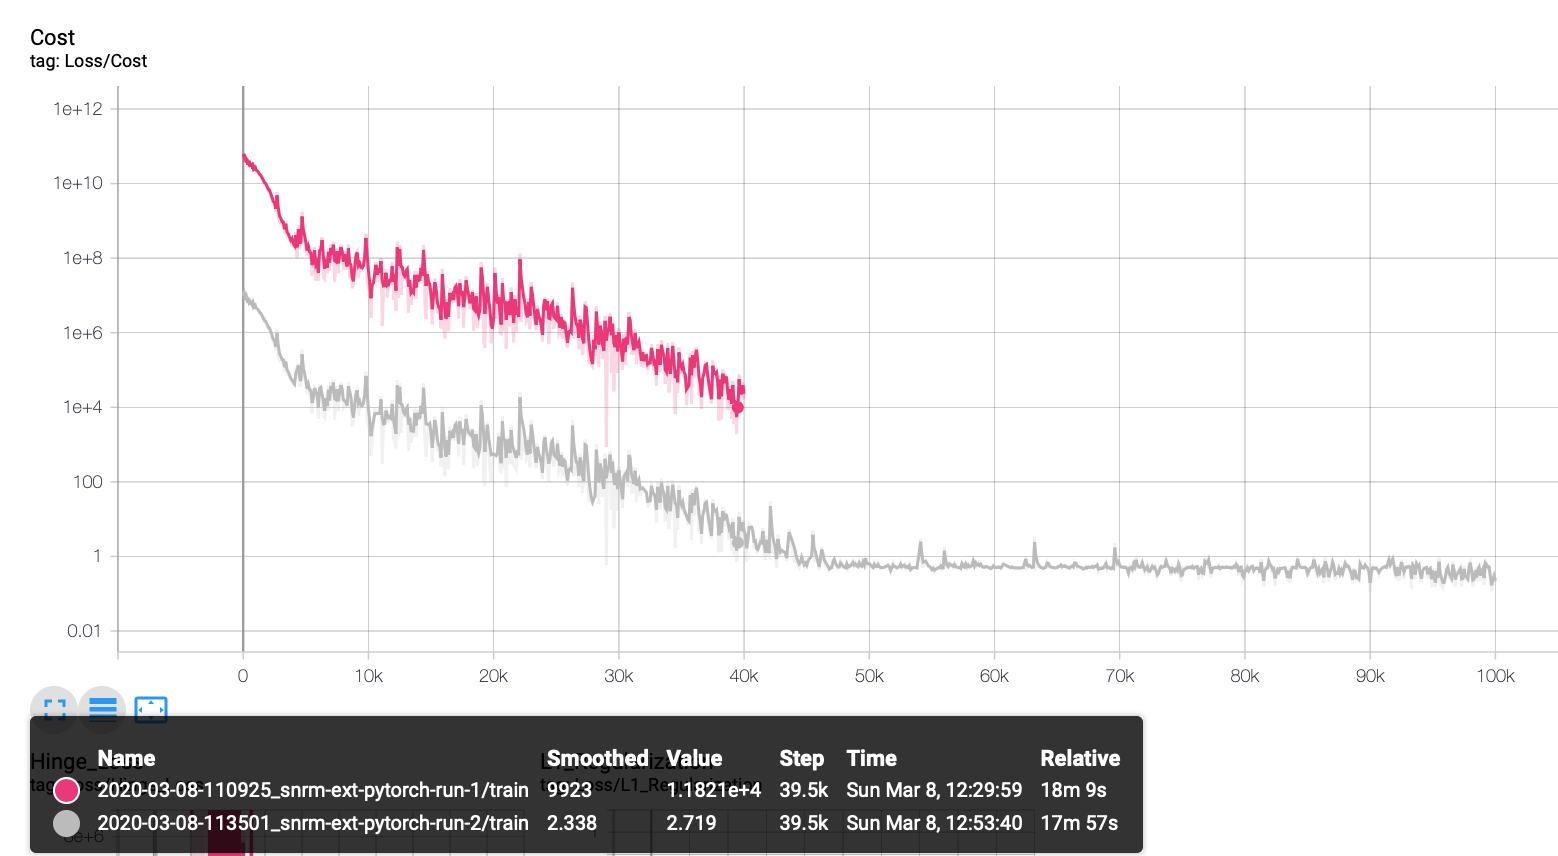
\includegraphics[trim=0.5cm 5cm 1cm 0.5cm,clip=true,width=\textwidth]{Bildschirmfoto_2020-03-08_relu-only-last_1.png}}
    \subcaption{Cost function of two runs with different regularization term $\lambda$ values}
    \label{fig:2020-03-08:relu-only-last:cost-fn}
\end{subfigure}
\begin{subfigure}[b]{0.45\textwidth}
    \centering
    \frame{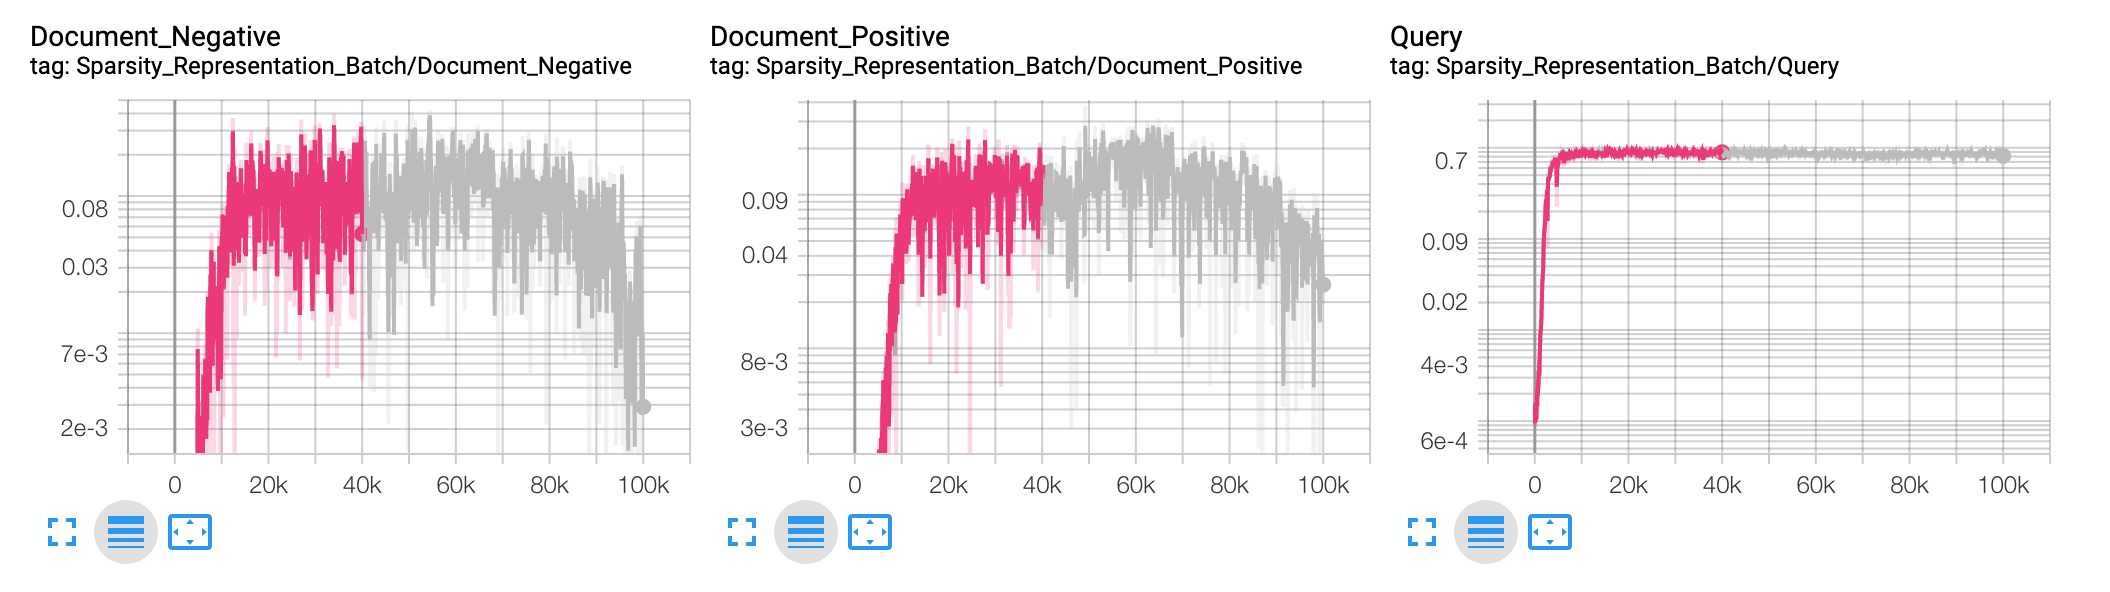
\includegraphics[trim=48.5cm 1cm 1.5cm 0.5cm,clip=true,width=\textwidth]{Bildschirmfoto_2020-03-08_relu-only-last_2.png}}
    \subcaption{Two runs with different regularization term $\lambda$ values show a non-controllable course of representation sparsity for query batches. After a few steps the query sparsity reaches about 0.70 and stayed there.}
    \label{fig:2020-03-08:relu-only-last:sparsity-query-repr}
\end{subfigure}
\hspace{0.042\textwidth}
\begin{subfigure}[b]{0.45\textwidth}
    \centering
    \frame{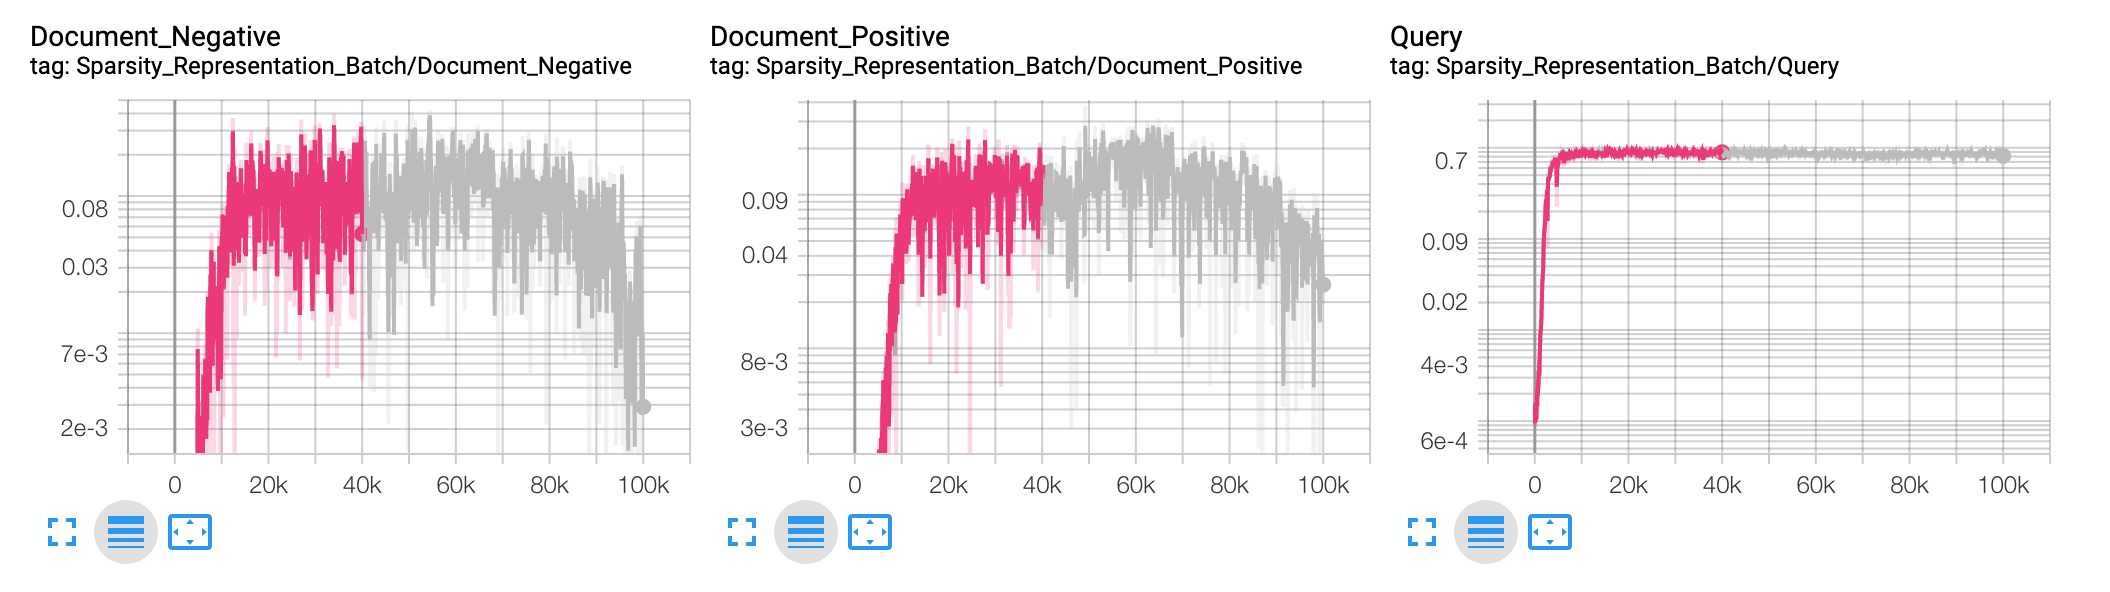
\includegraphics[trim=24.5cm 1cm 25.5cm 0.5cm,clip=true,width=\textwidth]{Bildschirmfoto_2020-03-08_relu-only-last_2.png}}
    \subcaption{Two runs with different regularization term $\lambda$ values show a non-controllable course of sparsity for document batches. The document sparsity shows much variation and a quite lower value of about 0.05 on average.}
    \label{fig:2020-03-08:relu-only-last:sparsity-doc-repr}
\end{subfigure}
% Remove the [...] argument if the original caption should be used in the figure list.
\caption[Costs function and non-controllable sparsity of two runs with different values of regularization term $\lambda$ of a model comprising sum reduction for hinge loss' logits computation, no dropout and ReLu only after the last layer]{Cost function approaching approx. 1 and non-controllable representation sparsity of query and document batches for two runs with different regularization term $\lambda$ values of a model comprising no dropout, mean reduction instead of sum reduction for the hinge loss' logit computation and a ReLu activation function only after the last convolution layer}
\label{fig:2020-03-08:relu-only-last:cost-fn-query-doc-repr-sparsity} % \label has to be placed AFTER \caption (or \subcaption) to produce correct cross-references.
\end{figure}

On the other side, running the experiment with a ReLu activation function after each convolution layer
    and using the value 0 as the regularization term $\lambda$, leaded to a
    quick progression of the sparsity for both, query and document representations, to 1,
    without beeing able to control the sparsity
Two plots in Figure~\ref{fig:2020-03-08:relu-all:cost-fn-query-doc-repr-sparsity} illustrate
    that the sparsity reaches 1 just after a few thousand steps, but without using any
    L1 regularization, and hence, without any means of controlling the sparsity.

% image: 2020-03-08 all-relu zu sparse Problem Tensorboard Diagramm.pdf" all-relu
\begin{figure}[htbp]
\centering
% trim: left bottom right top
\begin{subfigure}[b]{0.45\textwidth}
    \centering
    \frame{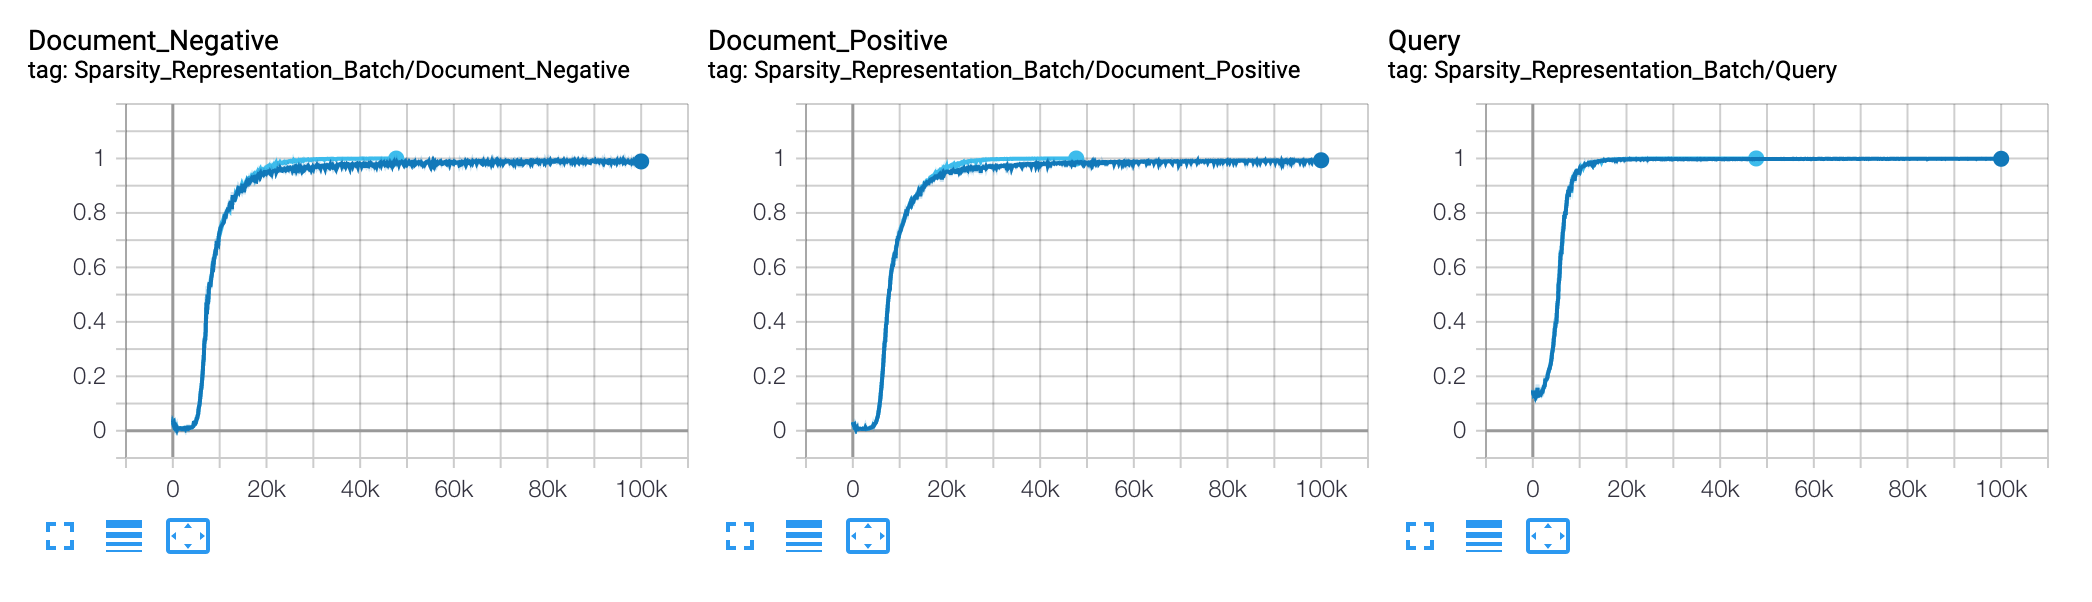
\includegraphics[trim=48.5cm 1.5cm 1cm 0.5cm,clip=true,width=\textwidth]{Bildschirmfoto_2020-03-08_relu-all_2.png}}
    \subcaption{The sparsity of query batches reaches 1 just after a few thousand steps, without beeing able to control the sparsity.}
    \label{fig:2020-03-08:relu-all:sparsity-query-repr}
\end{subfigure}
\hspace{0.042\textwidth}
\begin{subfigure}[b]{0.45\textwidth}
    \centering
    \frame{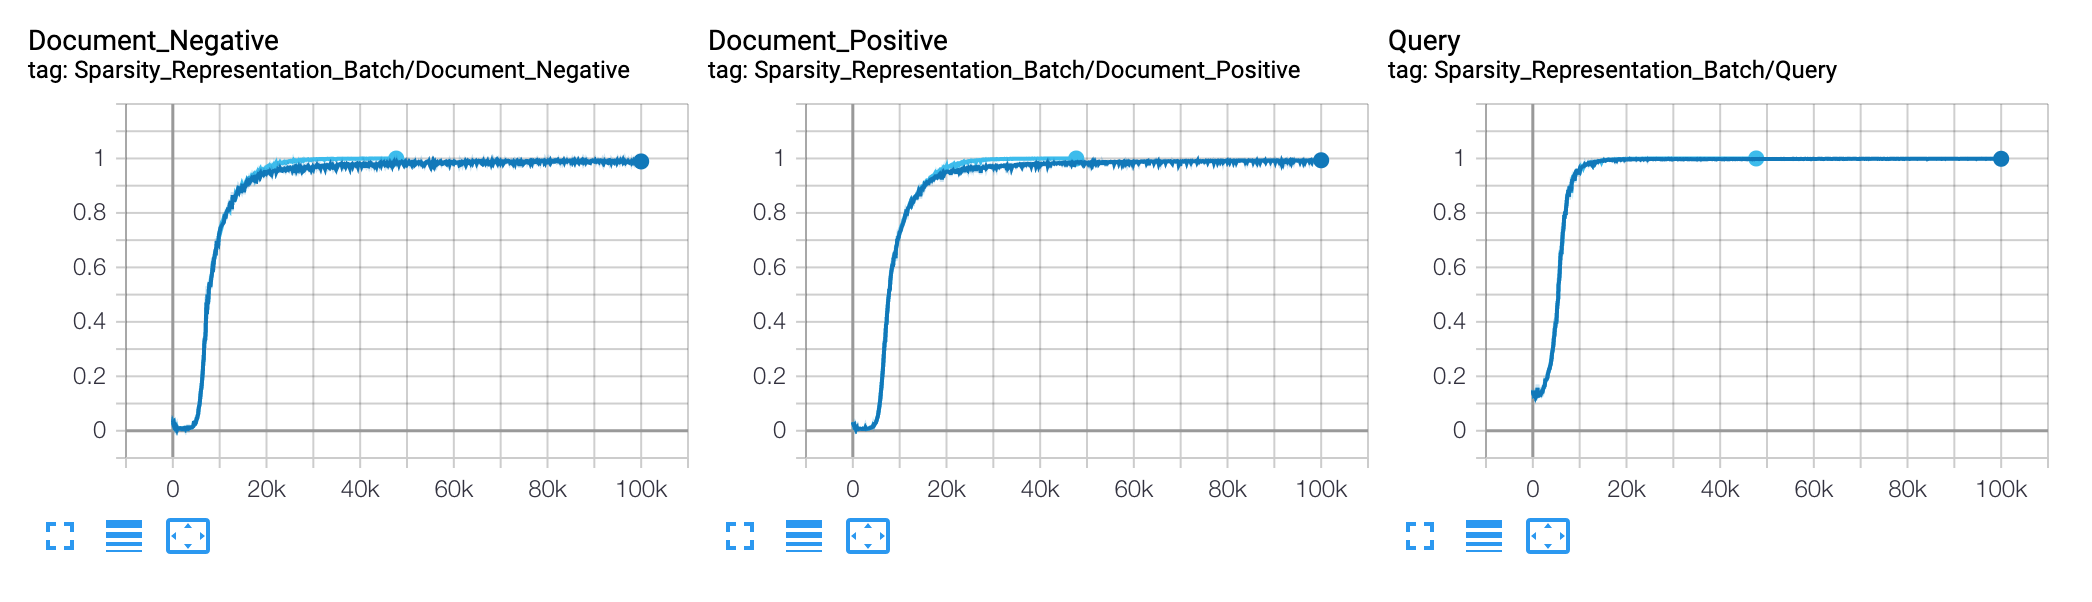
\includegraphics[trim=24.5cm 1.5cm 25cm 0.5cm,clip=true,width=\textwidth]{Bildschirmfoto_2020-03-08_relu-all_2.png}}
    \subcaption{The sparsity of document batches reaches 1 just after a few thousand steps, without beeing able to control the sparsity.}
    \label{fig:2020-03-08:relu-all:sparsity-doc-repr}
\end{subfigure}
% Remove the [...] argument if the original caption should be used in the figure list.
\caption[Non-controllable sparsity of a model comprising sum reduction for hinge loss' logits computation, no dropout, no L1 regularization and ReLu after all convolution layers]{Non-controllable representation sparsity of query and document batches of a model comprising no dropout, mean reduction instead of sum reduction for the hinge loss' logit computation, no L1 regularization and a ReLu activation function after all convolution layers}
\label{fig:2020-03-08:relu-all:cost-fn-query-doc-repr-sparsity} % \label has to be placed AFTER \caption (or \subcaption) to produce correct cross-references.
\end{figure}

\subsubsection*{Training with different training datasets}
After having discussed the work and the results, the model training was tried with two different
    training sets.
As already previously used for the reproduction of the TensorFlow implementation of SNRM, the training 
    dataset of the Advanced Information Retrieval lecture exercise files was used (\texttt{triples.train.tsv}).
% TODO is the following correct for triples.train.tsv from AIR lecture exercise?
%       Momentan ist bei uns einfach aus den top1000 von bm25 gesampled, 
%       was heißt dass die Dokumente zumindest irgendwas mit dem positive doc zu tun haben 
%       (und daher der unterschied kleiner ist). 
Negative documents are sampled from the top 1,000 from BM25 for the \texttt{triples.train.tsv} training file.
\todo{@Sebastian: Stimmt das in Bezug auf das AIR triples.train.tsv? Wie können wir es beschreiben? Wie kann ich mir das vorstellen, dass pos/neg docs was gemeinsam haben aufgrund v. sampling?}
That means, that the negative documents might have something in common with the positive documents,
    resp. the semantic difference between a positve and negative document passage might be smaller.
% TODO is this correctly written? :D should we add a link to the dataset or is description sufficient?
Therefore, two new training files, based on the MS MARCO dataset were generated, namely 
    one with a 50\% BM25 and 50\% collection sampling, and the other is to 100\% sampled from the collection,
    regarding the negative documents.
\todo{@Sebastian: Wie kann ich mir das nochmal genauer vorstellen, wie diese beiden Datasets generiert/gesampled werden?}
%       Aber er hat gesagt uniform sampling aus der Collection ist auch wichtig. 
%       Also hab ich jetzt mal zwei neue trainingsversionen erstellt 
%       (was das sampling der negativen docs betrifft):
%       50% bm25 + 50% collection sampling https://owncloud.tuwien.ac.at/index.php/s/iF37s8DOzvFjRkd
%       100% Collection sampling https://owncloud.tuwien.ac.at/index.php/s/Uk2n9pRxCigt6Dd
% TODO link to owncloud is invalid now/deleted, should we mention it here anyway?
\todo{@Sebastian: die zwei Datasets, die du generiert hast, sind mittlerweile nicht mehr auf OwnCloud, d.h. Verlinkung macht keinen Sinn. Reicht die Beschreibung bzgl. diesen Datasets?}
When comparing the Tensorboard diagramms for the model training, the two new training sets,
    did not change the course of the sparsity, compared to using the \texttt{triples.train.tsv} dataset.
A comparison of the query and document representation sparsity for a run without any L1 regularization
    and with ReLu activation functions only on the last layer,
    but with the two different training datasets
    (50\% BM25 and 50\% collection sampling, 100\% collection sampling),
    is plotted in Figure~\ref{fig:2020-03-10:relu-only-last:query-doc-repr-sparsity}.
It is not difficult to recognize that the diagrams look very similar to the ones in 
    Figure~\ref{fig:2020-03-08:relu-only-last:cost-fn-query-doc-repr-sparsity}.

% image of 2020-03-10_tensorboard_log_uniform_and_50_50 (tensorboard file) ?
\begin{figure}[htbp]
\centering
% trim: left bottom right top
\begin{subfigure}[b]{0.45\textwidth}
    \centering
    \frame{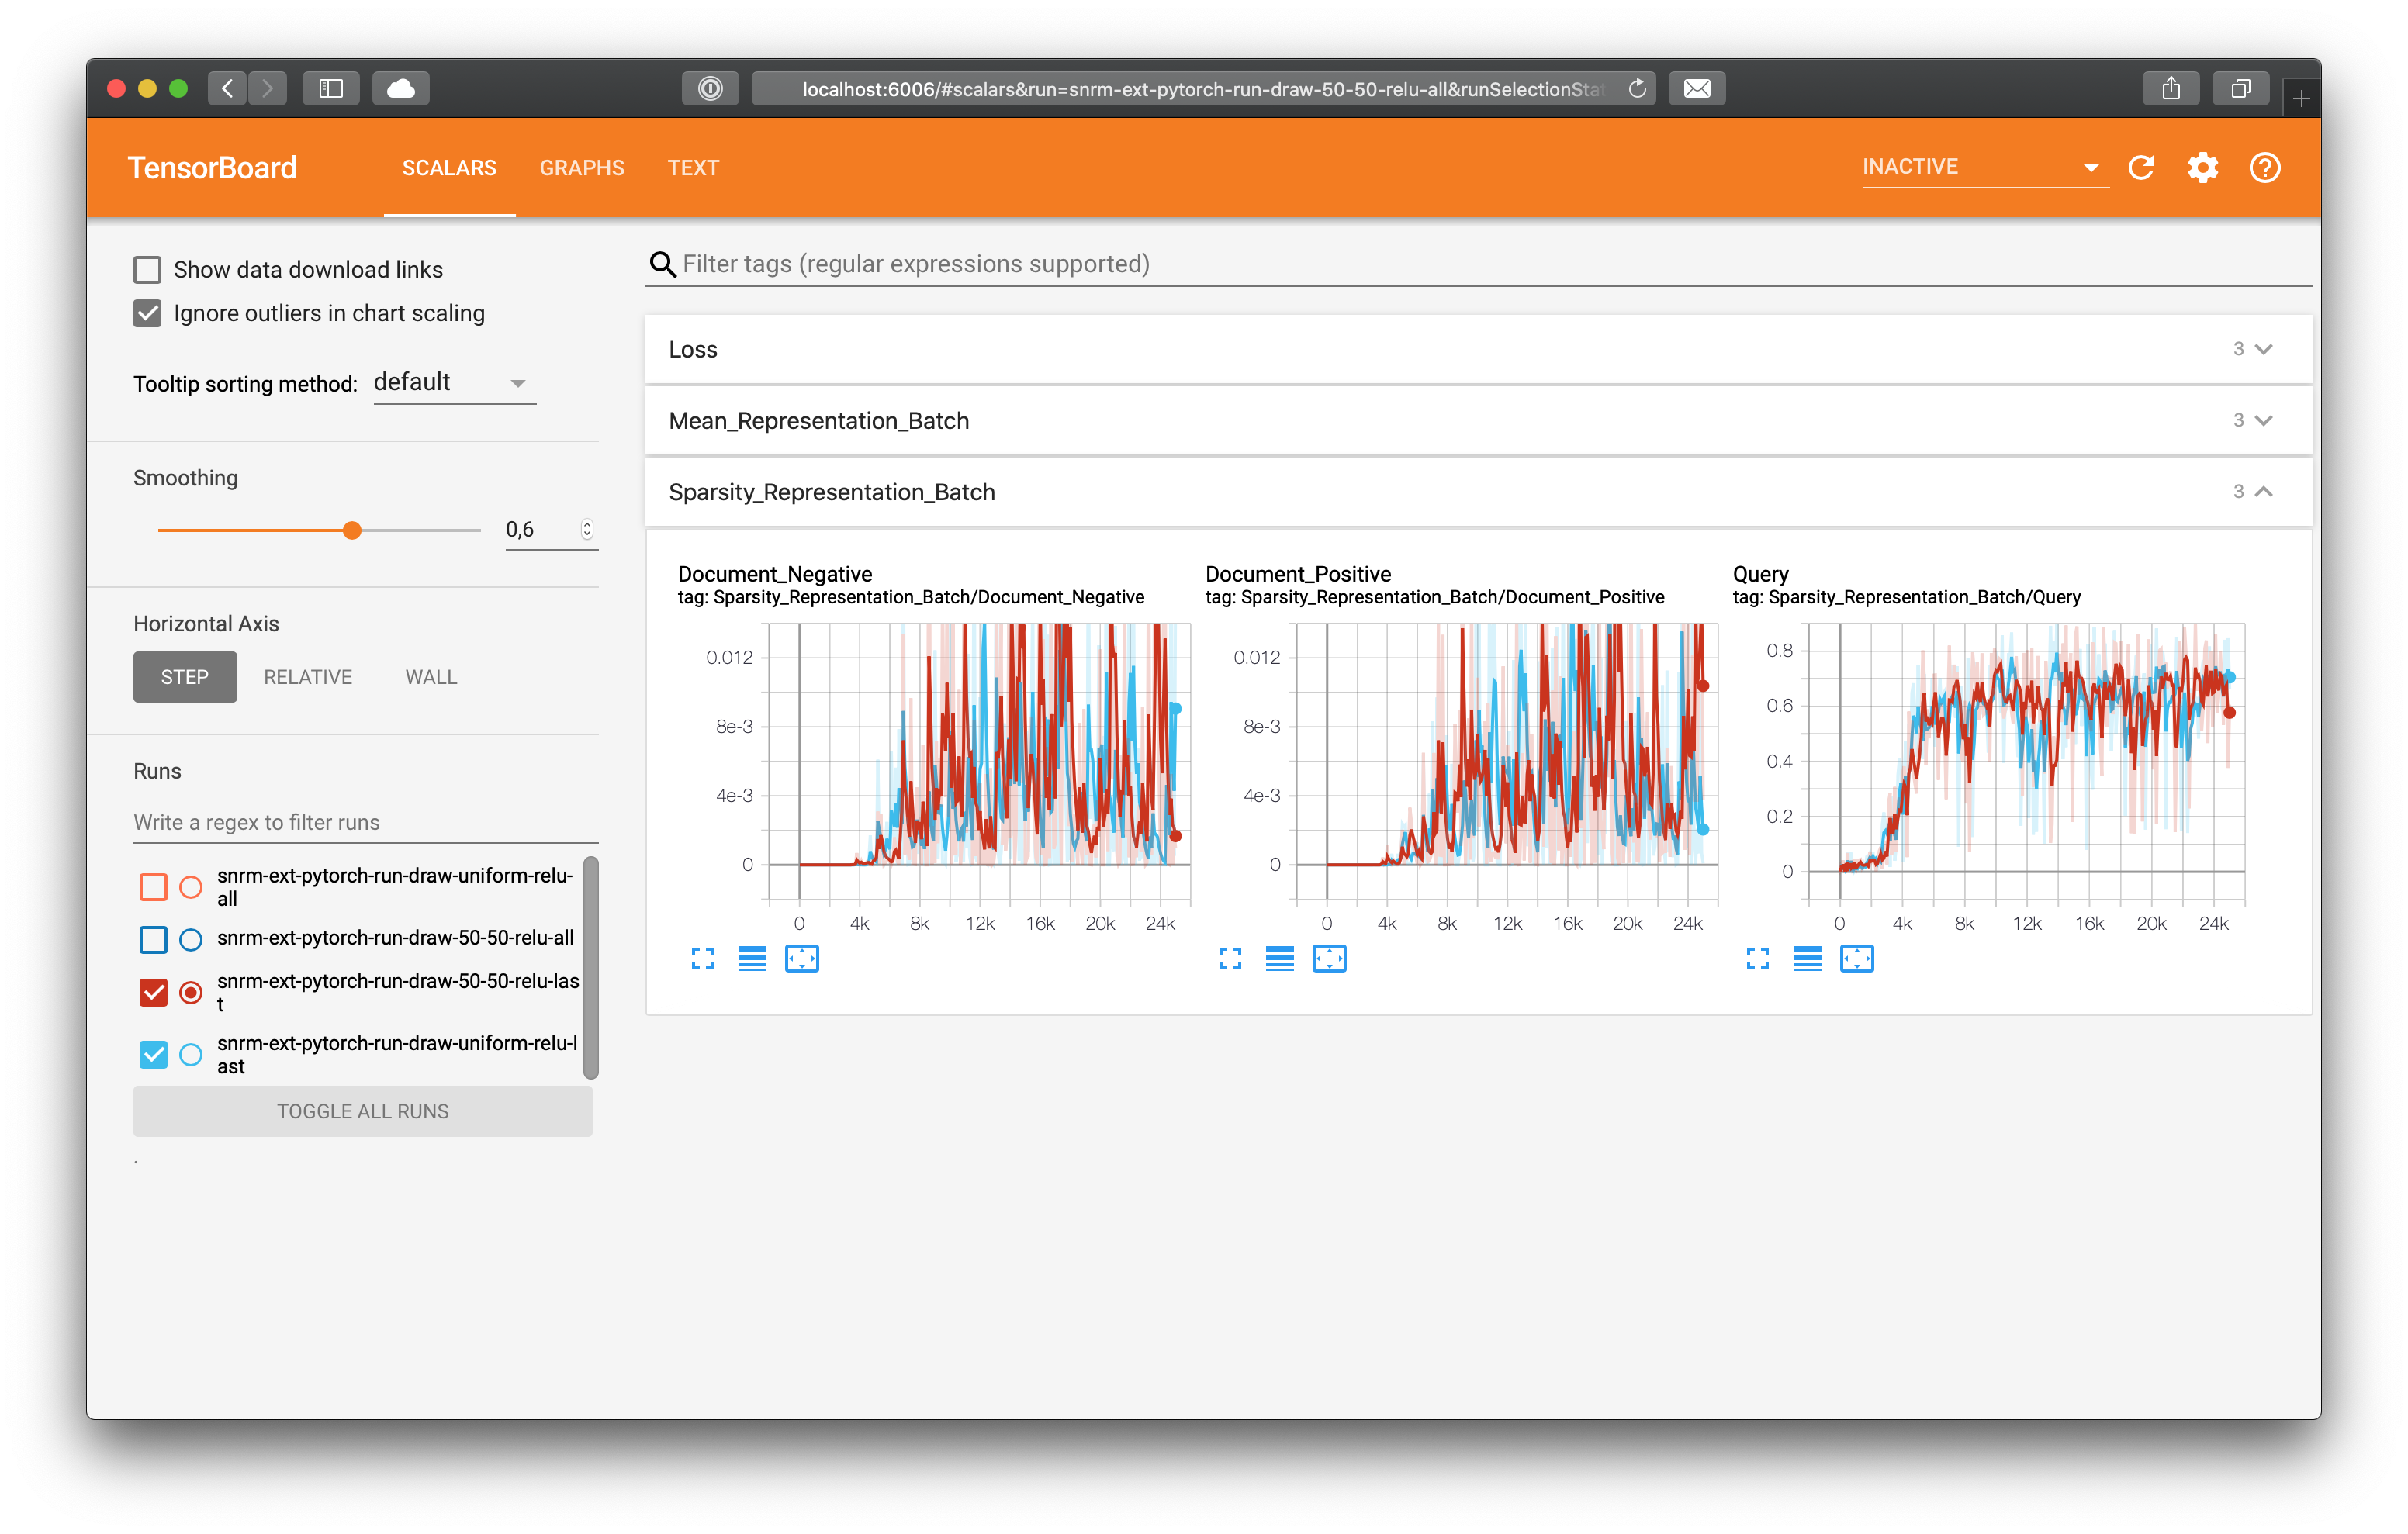
\includegraphics[trim=78.2cm 25cm 6.8cm 25cm,clip=true,width=\textwidth]{Bildschirmfoto_2020-09-29_relu-only-last_1.png}}
    \subcaption{Two runs with a different training dataset for query batches. After a few steps the query sparsity reaches about 0.60 and varied there a bit.}
    \label{fig:2020-03-10:relu-only-last:sparsity-query-repr}
\end{subfigure}
\hspace{0.042\textwidth}
\begin{subfigure}[b]{0.45\textwidth}
    \centering
    \frame{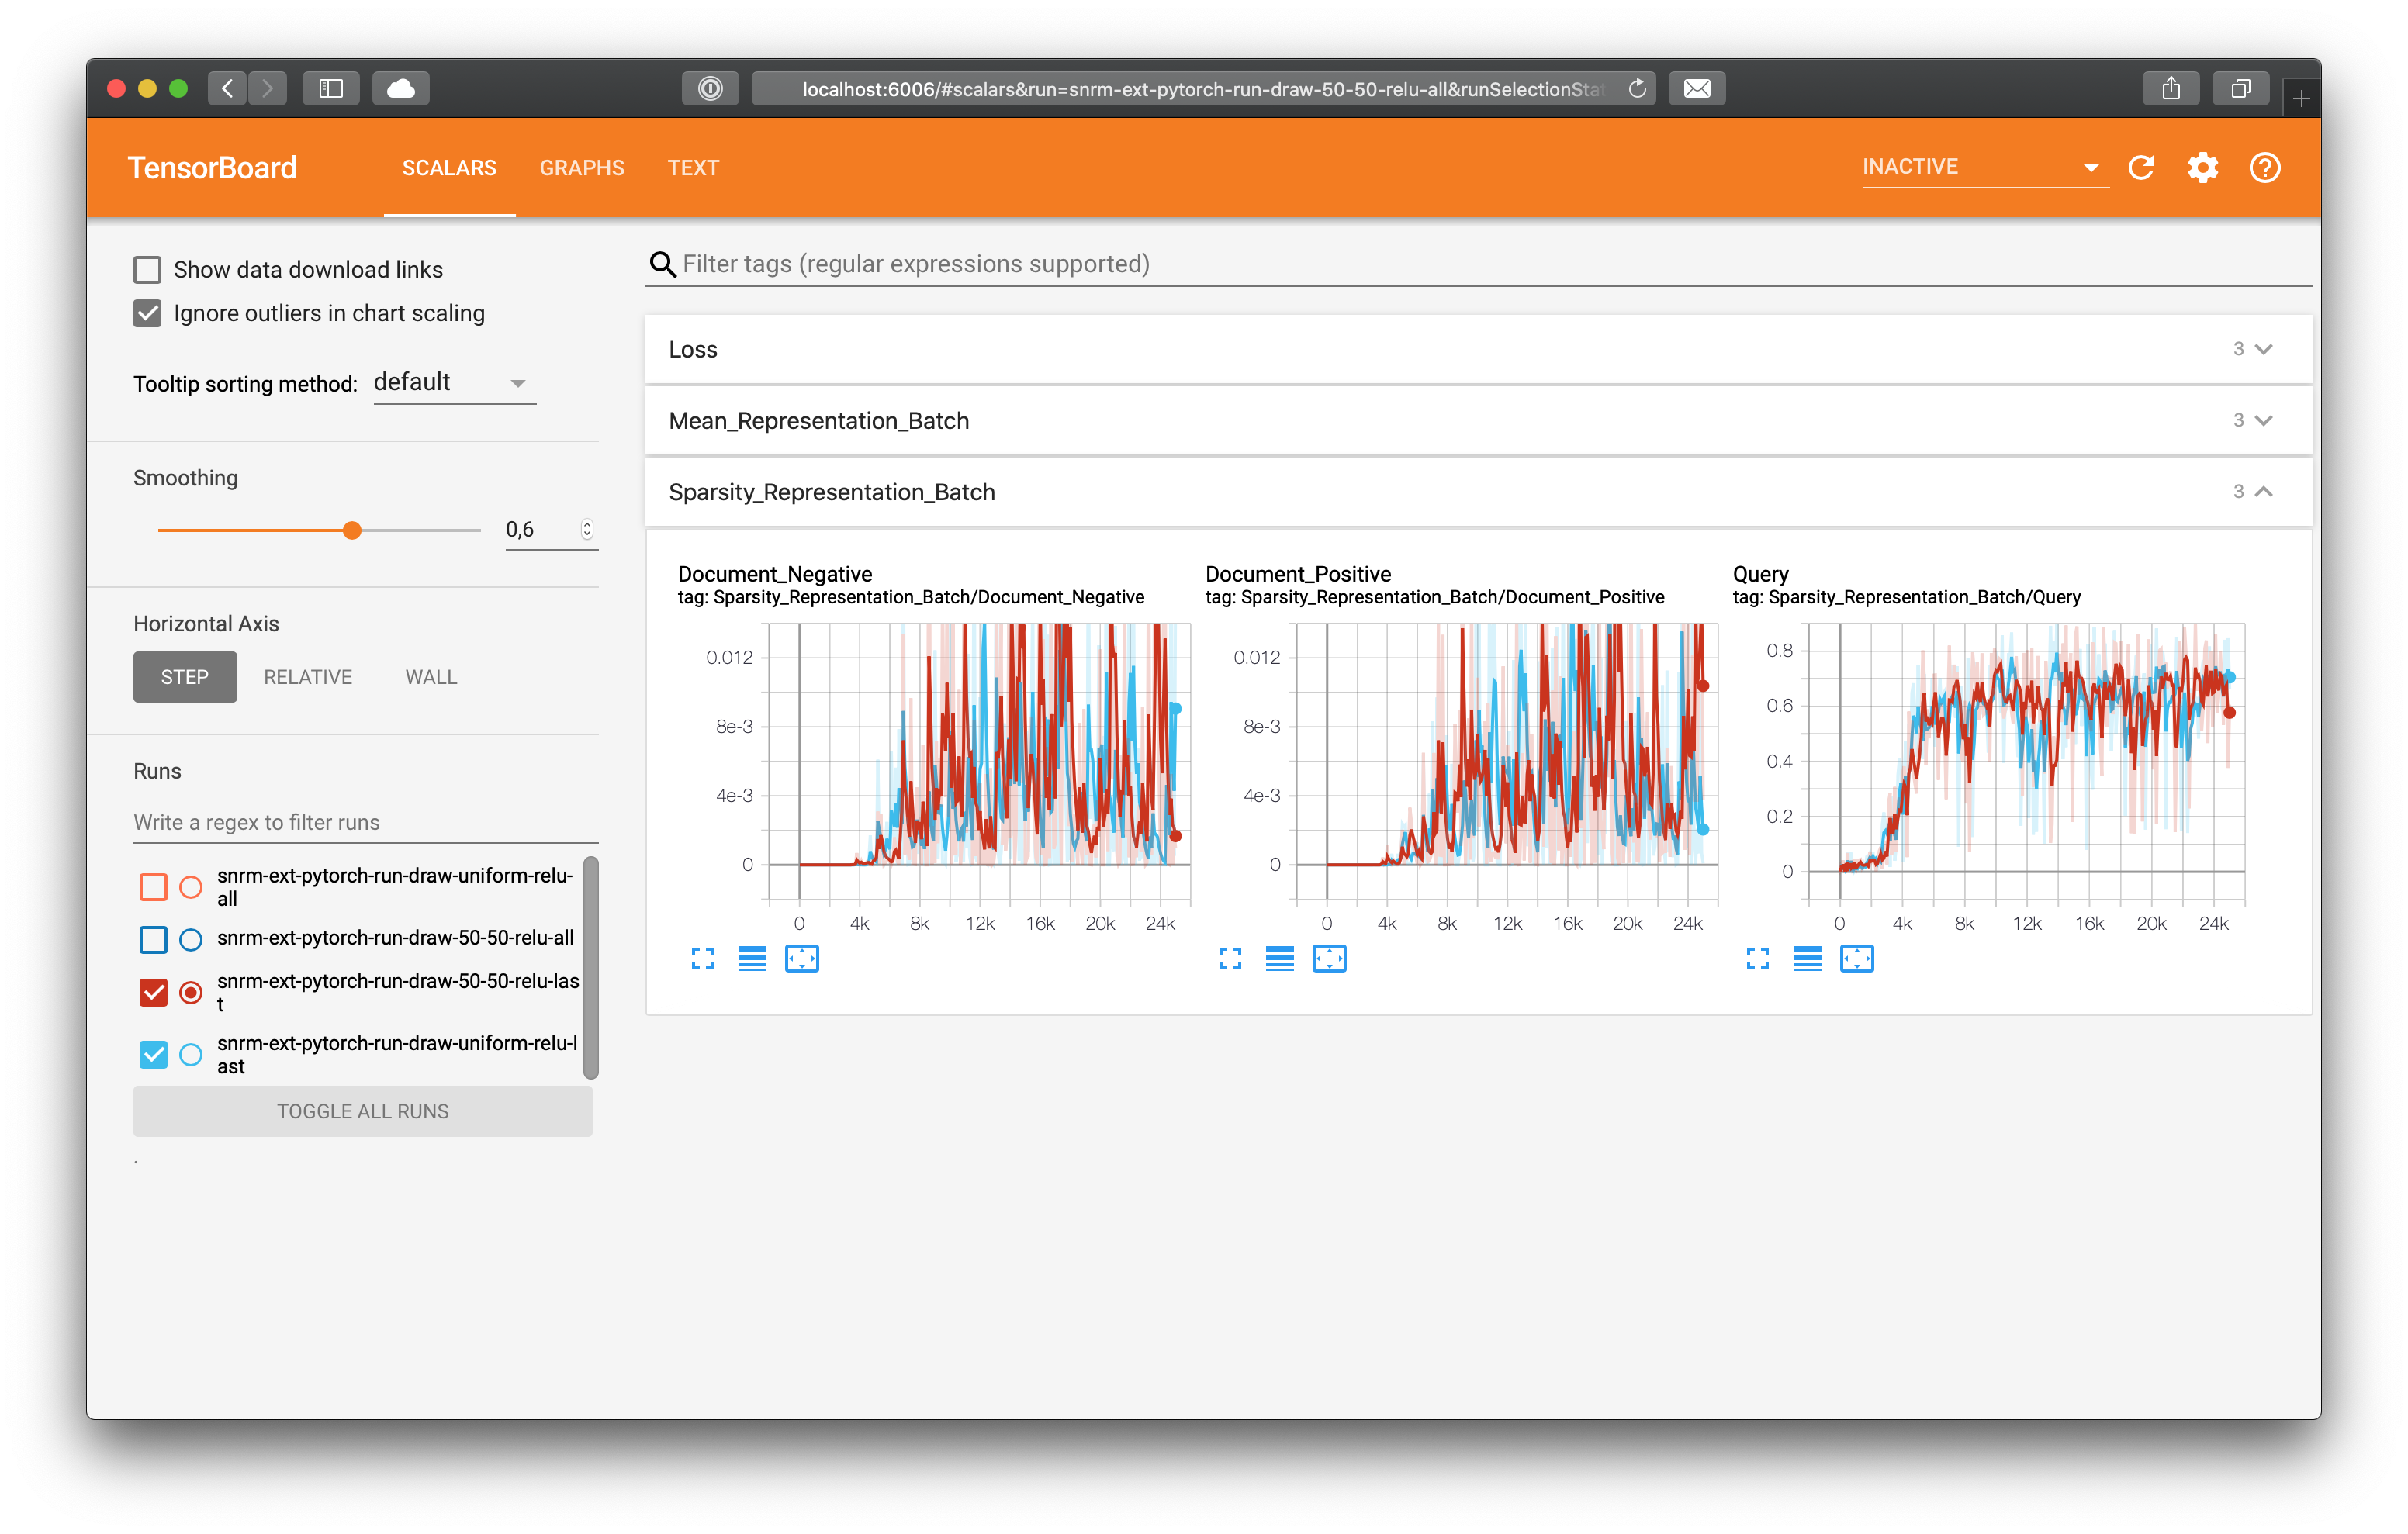
\includegraphics[trim=54.2cm 25cm 30.8cm 25cm,clip=true,width=\textwidth]{Bildschirmfoto_2020-09-29_relu-only-last_1.png}}
    \subcaption{Two runs with a different training dataset for document batches. The document sparsity varies much and has an average sparsity of about 0.006.}
    \label{fig:2020-03-10:relu-only-last:sparsity-doc-repr}
\end{subfigure}
% Remove the [...] argument if the original caption should be used in the figure list.
\caption[Sparsity of two different runs with different training dataset (50\% BM25 and 50\% collection sampling, 100\% collection sampling) of a model comprising sum reduction for hinge loss' logits computation, no dropout, no L1 regularization and ReLu only after last convolution layer]{Course of sparsity of two runs with different training dataset (red is drawn 50\% from BM25 and 50\% collection sampling, blue is 100\% collection sampling) of query and document batches of a model comprising no dropout, mean reduction instead of sum reduction for the hinge loss' logit computation, no L1 regularization and a ReLu activation function only after the last convolution layer}
\label{fig:2020-03-10:relu-only-last:query-doc-repr-sparsity} % \label has to be placed AFTER \caption (or \subcaption) to produce correct cross-references.
\end{figure}

\subsubsection*{Changing the L1 regularization with separated regularization terms}
In another approach was tried to control the representation sparsity and to reach for documents a similar
    sparsity than for queries.
Instead of calculating a L1 regularization together for a query, a positive and a negative document 
    representation batch and controlling the sparsity with one regularization term $\lambda$,
    it was tried to separate the L1 regularization for queries and documents.
Therefore, two regularization terms were introduced, namely $\lambda_{doc}$ and $\lambda_{query}$,
    which should control their respective L1 regularizations.
The document L1 regularization is calculated based on a positive and a negative document representation batch,
    and its impact should be controlled with the document regularization term $\lambda_{doc}$.
Whereas, the query L1 regularization is equal to the query representation batch, times the 
    query regularization term $\lambda_{query}$.
Then, the query and document L1 regularization tensors are summed up, a sum reduction is applied,
    and the L1 regularization is calculated by taking the mean.
The code in Listing~\ref{comparison-l1-regularization-before-after} shows the different calculation of the L1 regularization before the approach
    of controlling the query and document sparsity separately, and how it is afterwards.

\begin{lstlisting}[language=Python,frame=single,breaklines=true,float=tbh,caption=Comparison of the L1 regularization calculation before and after separating it on query and documents,label=comparison-l1-regularization-before-after]
##### BEFORE #####

l1_regularization = torch.mean(
        torch.sum(
                input=torch.cat(tensors=(
                    q_repr, doc_pos_repr, doc_neg_repr),
                    dim=1), 
                dim=1))

# l1_regularization (scalar)
l1_regularization = torch.mul(l1_regularization, 
                              regularization_term)

##### AFTER #####

# separate regularization terms for query and documents
doc_reg_term = config.get('doc_reg_term') 
q_reg_term = config.get('q_reg_term')

# separate l1 regularization for query and document
l1_regularization_docs = (doc_pos_repr + doc_neg_repr) * 
                         doc_reg_term 
l1_regularization_query = q_repr * q_reg_term

# l1 regularization (scalar)
l1_regularization = torch.mean(
        torch.sum(
            input=(l1_regularization_docs + 
                   l1_regularization_query), 
            dim=1))
\end{lstlisting}

Inspecting the model's TensorBoard diagrams after modifiying the L1 regularization showed,
    that the modification was not able to change the course of the sparsity significantly.
In some of those runs the cost function stayed on relatively large values (e.g. 1e+6)
    and stayed there with a few variations.
% TODO maybe add an image of tensorboard_snrm_2020-03-15.zip (tensorboard file)
When for the cost function only the L1 regularization without the hinge loss was used,
    the sparsity also did not change much.
Rather than the cost function approaching the value 0, it settled down to a value
    around 200.
% TODO maybe add image of 2020-03-17_tensorboard_snrm_only_l1_reg 2 (tensorboard file)    

\subsubsection*{Adding a bias to convolution layers}
After that, it was tried to use a bias vector for the convolution layers.
In the original SNRM TensorFlow code a comment indicated, that they did not use biases,
    although they created variables for them, but did not use them.
Note, that the SNRM PyTorch model definition above, shows already the \texttt{nn.Conv2d} 
    layer's argument \texttt{bias=True}.
With a bias vector and by using for the cost function only the L1 regularization separated 
    for query and documents without the hinge loss,
    the course of the sparsity changed and approached the value 1 quickly after a few thousand 
    training steps.
Also the cost function neared 0 after a few thousand training steps.
% TODO maybe add image of 2020-03-18_tensorboard_reduced_dims_bias 2 (tensorboard file)

\subsubsection*{Attempt to control representation sparsity}
With that result, it was tried to control the sparsity with different values for 
    the query and document's regularization terms $\lambda_{doc}$ and $\lambda_{query}$.
The neural network's number of units per hidden layer was configured to 10, and three 
    hidden layers were used.
Without a L1 regularization, the sparsity was lower, compared to using one,
    and the course of the sparsity was controllable with the regularization terms.
But even small changes in a L1 regularization term causes the sparsity to rise too fast to 1.
Besides that, changes in one of the L1 regularization terms, e.g. $\lambda_{doc}$,
    also influences the sparsity of the other entity, i.e. the query.
The cost functions during the experiments neared 0.5 after a few thousand steps and stayed 
    there with few variations.\\
In these training runs, the sparsity varied, but it was possible to save a PyTorch model    
    with a sparsity of about 0.97, create an inverted index with it, and evaluate it.
% TODO maybe add images of tensorboard_2020-04-06.zip (tensorboard file)
An analysis of the inverted index showed there were 807,360 documents added.
The minimum and maximum number of documents per latent term dimension was 
    1 document resp. 807,360 documents.
That is, for at least one latent term dimension all document were relevant,
    and this although the stopwords were filtered.
Further, the mean number of documents per latent term dimension was 13,772.70, 
    the median was 1013, and the 0.90-quantile 33,174.

A retrieval of relevant documents for evaluation queries was not possible,
    because of the large number of possibly relevant documents for some 
    latent term dimensions.
The retrieval script was modified in a way to skip latent term dimensions with
    a large amount of documents assigned.
And even with that adjustment, there were more often at least 50,000 documents per 
    latent term dimension returned.
As a consequence, the documents' representations still were not sparse enough, although 
    the document sparsity in TensorBoard during training approximately 0.98 was for documents.
Multiple evaluation query representations had postive coefficients
    for the same latent term dimensions, for which also all documents are relevant.
The information retrieval metrics still were non-positive.
Obviously, the model did not learn the specific of documents and queries, but general
    concepts, that are suitable for many or all.

After this test and analysis, further model trainings and experiments were carried out.
When modifying the neural network, to use variations of either two or three hidden layers 
    with 100 or 300 neurons each, 
    the course of the sparsity increased quite quick to 1, without using any L1 
    regularization term.
Therefore, no L1 regularization would be necessary for such a neural network,
    and the sparsity was already too high after several ten-thousand training steps,
    making the model training useless.

Additionally, it was tried to switch to a different tokenizer resp. word splitter.
Previously, the AllenNLP's \texttt{JustSpacesWordSplitter} was used,
    but it was also tried to use the AllenNLP \texttt{SpacyWordSplitter} with the 
    language model \texttt{en\_core\_web\_lg}.
Despite changing the tokenizer, the sparsity progression was not significantly different
    compared to previous runs.

\subsubsection*{Changing convolution layers' parameter initialization}
Further, the already employed TensorBoard reporting was extended to create histograms
    of the model's weights and bias values during training, to investigate how the parameter
    values are distributed and vary.
These histograms allowed to monitor the course of parameter value changes.
So far, the PyTorch model' weights were initialized just like in the original SNRM TensorFlow
    implementation with random values of the normal distribution.
The TensorBoard histograms of weight values looked bell-shaped and there mean did not change much.
However, in the bias histograms an initial bell curve was dismantled, and the values 
    varyied and their values were more distributed.
Looking only at the model's course of weight and bias changes, it seemed that the model
    primarily adjusts its bias without changing the neurons' weights much.
% TODO should we add histograms of learned parameters?
% "Bildschirmfoto 2020-04-11 um 15.56.06.png“ 
% "Bildschirmfoto 2020-04-11 um 16.21.13.png“
% or create new images from a new run...

This insight led to thinking about different methods of parameter value initialization.
Obviously, PyTorch does by default for convolution layers a 
    "He initialization" (\texttt{torch.nn.init.kaiming\_uniform\_}) for its weights,
    and intializes the bias from a uniform distribution (\texttt{torch.nn.init.uniform\_}),
    according to the \texttt{conv.py} convolution class's function
    responsible for resetting parameters
    \footnote{PyTorch v1.4 code of convolution class with \texttt{reset\_parameters} function \url{https://github.com/pytorch/pytorch/blob/v1.4.0/torch/nn/modules/conv.py\#L49}}.\\
Next, it was tried to use PyTorch's default initializatoin method for convolution layers,
    and the MSMARCO passage ranking training data set \texttt{train.triples.small.tsv} from Microsoft's 
    GitHub respository
    \footnote{MSMARCO training dataset \texttt{train.triples.small.tsv} on GitHub \url{https://github.com/microsoft/MSMARCO-Passage-Ranking}},
    due to more available training data.
Training with a neural network architecture with three hidden layers with 100 or 300 neurons per layer,
    and with 10,000 output neursons, showed that the sparsity was controllable again with 
    the query and document regularization terms $\lambda_{doc}$ and $\lambda_{query}$.
However, the course of the sparsity behaved very differently than before, due to frequent variations,
    and a slower progression.
Also, the cost function does not start with such large values than before (e.g. 2e+6),
    but with values near 0.5.
Though, the cost function varied between 0.5, there was no pattern showing that the function moves 
    towards the value 0, despite training for about 400,000 training steps.
% TODO maybe add image of after_train_2020-04-18_230538 (tensorboard file)
%       sparsity, histograms?
%       i.e. tf-log/2020-04-18-203850_snrm-ext-pytorch-run-1-draw-uniform-layers-300-100-300-10k-default-weight-init-l1-reg-2e-8-2e-12/train
%            tf-log/2020-04-26-164458_snrm-ext-pytorch-run-1-train-triples-layers-300-100-300-1k-l1-reg-1e-8-1e-12/train

Saving a model with a suitable sparsity ratio (e.g. 98\%) however showed that the information retrieval
    evaluation metrics still were non-positive.
The same challenges as before remained, that is an improper sparsity ratio of evaluation queries and 
    a too large number of relevant documents per latent term dimension.
Obviously, the model was not able to learn semantic word relationships and conecpts 
    from the training dataset.\\
These results concluded the practical part of the thesis, regarding the reproducibility of the 
    standalone neural ranking model (SNRM) of
    Zamani et al. \cite{zamani:2018:from-neural-reranking-to-neural-ranking}
    with the MSMARCO passage ranking dataset, 
    and the migration of SNRM from the Python library TensorFlow to PyTorch.

% TODO which source code should be added to the implementation section? github reference enough?
%      certain parts of model?